\setlength\abovedisplayskip{0pt} \setlength\belowdisplayskip{0pt}
\setlength\abovedisplayshortskip{0pt} \setlength\belowdisplayshortskip{0pt}

\chapter{Fundamenta\c{c}\~ao Te\'orica}
\label{theorycap}

Neste capítulo serão discutidos e explicados todos os conceitos e 
fundamentos necessários para a compreensão da proposta 
feita nesse trabalho, assim como a abordagem que será utilizada 
para a implementação de todos os componentes que juntos vão compor 
o motor de jogos que será o objeto de estudo.

\section{Modelagem Orientada a Dados}
\label{secdataorienteddesign}

A modelagem orientada a dados (do inglês: \textit{Data Oriented Design}) é 
uma forma de codificar os programas que propõe uma mudança no foco da 
implementação: ao invés de se focar no código, o foco deve estar nos 
dados. Apesar do termo "orientação a dados"\ ter sido usado apenas recentemente, 
a utilização dos conceitos dessa técnica já têm sido usados há muito mais tempo 
do que a introdução do termo.

Orientação a dados foi introduzido por John A. Sharp~\cite{Sharp1980}, cujo objetivo 
era aumentar a eficiência do processador e da utilização da memória. Além disso, o autor 
cita que um dos objetivos dessa técnica de programação é facilitar a concorrência na 
execução dos programas. No seu trabalho é proposta uma metodologia de projeto que 
menciona outro conceito importante, o do fluxo de dados.

Ao se projetar um programa ou sistema, a primeira tarefa a ser feita é determinar o 
fluxo de dados necessários. Essa etapa consiste em determinar quais componentes do 
sistema requerem cada um dos diferentes tipos de dados presente neste, e também 
especificar quais são os componentes que geram novos dados. Depois que o fluxo de dados 
no sistema está completamente especificado, o próximo passo é descrever como os dados 
recebidos por cada componente são transformados nos dados que este componente precisa 
gerar. Sharp defende que qualquer programa pode ser descrito dessa maneira, a 
transformação de um dado conjunto de \textit{inputs} para um certo conjunto de 
\textit{outputs} requeridos.

Um exemplo é o trabalho de Chellappa et al.~\cite{chellappa2008write}, no 
qual é reconhecido o problema da velocidade de acesso à memória principal pelo 
processador, e para solucionar esse problema é dito que os dados de uma aplicação devem 
ser lidos na ordem apropriada. Otimizações feitas pelos compiladores são 
limitadas para o caso da leitura da memória, pois o que define o quão rápido 
os dados serão lidos são as estruturas utilizadas para armazená-los, 
algo que o compilador não é capaz de otimizar. 

Além disso é reconhecido pelos autores o fato de um \textit{cache miss} causar a perda de 
ciclos e, consequentemente, a perda de operações de ponto flutuante. Para demonstração do 
problema e sua solução através da reestruturação de código, são mostrados no artigo 
dois algoritmos diferentes que têm seus desempenhos aprimorados após a mudança nas 
estruturas de dados utilizadas.

Uma das premissas do DOD é ter preferência a leitura sequencial dos dados. Para atingir 
isso, os objetos pertencentes ao domínio do problema são representados por 
identificadores únicos que são utilizados para acessar suas propriedades. Essas 
propriedades são \textit{arrays} de dados que são armazenados na memória de maneira 
contígua, e para utilizar essa técnica de maneira eficiente, é essencial administrar 
esses \textit{arrays} das propriedades para garantir que permaneçam contíguos conforme 
novos dados são adicionados e removidos~\cite{Fontana2017}.

Ao se modelar o código através de uma abordagem orientada a objetos, esta modelagem 
é centrada em volta do problema e da sua solução. Os objetos, que não são coisas reais, 
mas sim o resultado das soluções para o problema apresentado, manipulam apenas os dados 
necessários para representá-los sem nenhuma consideração pelo hardware, pelos 
padrões de dados reais ou de quantidades, por isso essa abordagem permite uma rápida 
prototipagem dos programas pois essas soluções podem ser escritas diretamente da 
modelagem para o código~\cite{fabiandod}.

DOD utiliza uma abordagem diferente, prevendo onde os dados são mais vistos ou 
esperados através da determinação do fluxo de dados, utiliza o caso 
mais provável para direcionar a escolha do algoritmo. Com isso, ao se utilizar essa 
abordagem pode-se separar os dados mais utilizados dos menos utilizados de tal forma 
que estes não sejam desnecessariamente carregados da memória. Não 
saber como esses dados estão armazenados na memória pode ser 
prejudicial para o desempenho do programa.

A figura~\ref{oodvsdod} apresenta duas maneiras diferentes de se ler dados da memória, 
a primeira ocorre com a programação orientada a objetos, na qual os dados não são lidos 
de maneira contígua. A sequência de chamadas da figura ilustra o modo como as 
propriedades de um objeto são lidas de maneira intercalada nesse esquema de dados. 
Caso uma rotina necessite, por exemplo, de um dado contido em C, é necessário manter 
a referência de A e de B na memória. Isso geralmente ocorre em POO, em casos nos quais 
objetos possuem ponteiros para objetos de outras classes. Se os dados contidos em C não 
estivessem atrelados a B, que por sua vez está atrelado a A, a leitura de dados seria 
mais eficiente. 

Na figura~\ref{fig:dod} há uma separação do objeto em componentes diferentes, e 
componentes do mesmo tipo são agrupados juntos na memória, independentemente do objeto 
de qual vieram. Essa organização resulta em blocos largos de dados homogêneos, 
permitindo o uso eficiente de memória através processamento de dados contíguos. 

\begin{figure}[h!]
    \centering
    \captionof{figure}{Orientação a objetos vs. Orientação a Dados. Duas maneiras 
    diferentes de se ler os dados da memória.}
    \begin{subfigure}[b]{0.35\textwidth}
        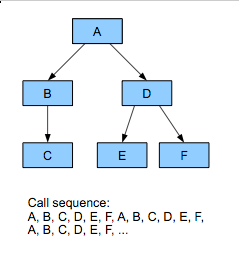
\includegraphics[width=\textwidth]{../figuras/objectreadingorder}
        \caption{Orientação a Objetos}
        \label{fig:ood}
    \end{subfigure}
    \begin{subfigure}[b]{0.35\textwidth}
        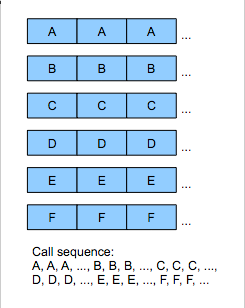
\includegraphics[width=\textwidth]{../figuras/dodreadingorder}
        \caption{Orientação a Dados}
        \label{fig:dod}
    \end{subfigure}
    \par\medskip
    Adaptado de: <http://gamesfromwithin.com/data-oriented-design>. Acesso em: 27/05/2017.
    \label{oodvsdod}
\end{figure}

\medskip

Outra proposta do DOD, além da divisão dos objetos em diferentes 
componentes, é utilizar a ordenação de dados ao invés de armazenar 
o estado de um objeto. O motivo de evitar o armazenamento do estado 
de um objeto se deve pela necessidade de condicionais para checar 
esse estado. A figura~\ref{dodobjectstate} demonstra um exemplo de 
ordenação de dados, em que os objetos de uma cena foram divididos 
entre os renderizáveis, e os não renderizáveis, desta maneira não há 
necessidade de verificar se o objeto está eleito para renderização 
no loop principal.

\begin{figure}[h!]
    \centering
    \captionof{figure}{Divisão de objetos entre os renderizáveis e os não renderizáveis
    (objetos fora do campo de visão do espectador).}
    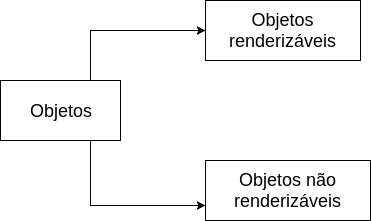
\includegraphics[width =\textwidth]{../figuras/dodobjectstate}
    \par\medskip
    Fonte: Autoria própria
    \label{dodobjectstate}
\end{figure}

O uso de condicionais dentro de um \textit{loop} pode causar 
\textit{branching}, que é o ato da troca da atual sequência de 
instruções do programa por uma outra sequência, caracterizando um 
desvio do comportamento padrão de execução das instruções em 
ordem~\cite{knuthart}. Tal desvio é causado pela execução de uma instrução que 
causa ramificação na execução do programa, instruções com condicionais 
são exemplos de instruções que causam \textit{branching}.

O \textit{branching} é um dos fatores que dificultam o uso de uma técnica conhecida 
por cache \textit{prefetching}, utilizada pelos processadores para aprimorar o 
desempenho, algumas instruções ou dados são buscados da memória principal e movidos 
para o cache antes que seja necessário usá-los~\cite{smith1982}. Para que o 
\textit{prefetching} ocorra, é necessário que o algoritmo responsável pela 
técnica preveja qual ramo será o executado. Caso a escolha esteja errada, 
o erro de previsão causa penalidades no desempenho, e o processador precisa 
despejar as instruções ou dados que haviam sido buscadas de 
antemão~\cite{tianprefetch}.

Se uma referência a um \textit{array} é precedida por uma instrução com 
condicionais, há dois problemas para se realizar o \textit{prefetching} dos 
dados do \textit{array}: o primeiro problema é que o teste condicional da 
instrução pode ser verdadeiro somente para um subconjunto do \textit{array} 
e realizar um \textit{prefetching} no \textit{array} poderia resultar na 
transferência desnecessárias de dados para o cache. O segundo problema é 
que o teste condicional pode estar impedindo o referenciamento de dados 
não existentes no \textit{array}, e realizar o \textit{prefetching} para 
esses dados poderia resultar em comportamento 
inesperado~\cite{vanderwieldataprefetch}.

Para evitar o uso de instruções com condicionais, principalmente em 
métodos que são utilizados com frequência, pode-se separar os dados entre 
aqueles que passam no teste condicional e aqueles que não passam, desta 
forma a verificação com condicionais se torna desnecessária, e o fluxo de 
execução das instruções não é interrompido por \textit{branching}.

O desvio excessivo da ordem de execução padrão de um programa 
também pode ser evitado tratando sempre o caso mais comum primeiro.
 Isso significa que, ao descrever uma transformação sobre um 
\textit{input} de dados, essa transformação deve levar em 
consideração qual será o caso mais comum para esse \textit{input}, 
em termos de estado e de quantidade. 

Em aplicações desenvolvidas com programação orientada a objetos, 
as transformações de dados geralmente são feitas através dos 
métodos implementados de cada classe. Esses métodos estão no 
escopo do objeto e por isso não possuem acesso aos atributos dos 
outros objetos da mesma classe. Consequentemente as instruções 
descritas nos métodos operam somente sobre os atributos do objeto 
que fez a chamada do método.

Essa abordagem é irrealista no contexto de jogos e aplicações 
gráficas, pois em poucas situações o caso mais comum será um 
único objeto. Se o caso mais
comum de \textit{input} para uma transformação é um conjunto 
de objetos, então essa transformação 
deve conter instruções que operam sobre o conjunto inteiro de 
objetos e somente sobre as propriedades que são realmente 
necessárias, otimizando o fluxo de instruções e o acesso à 
memória~\cite{fabiandod}. Transformações sobre um único objeto 
causam poluição desnecessária do cache quando estas precisam 
ser feitas sobre vários objetos em sequência, principalmente 
quando somente uma parcela dos atributos do objeto é 
necessária.

O esquema de armazenamento apresentado na 
figura~\ref{fig:dod} é um meio de se armazenar uma sequência de 
dados na memória conhecido como \textit{Structure of Arrays} (SoA), 
no qual os dados de um registro são separados em \textit{arrays} 
paralelos, um para cada atributo do registro. Desta maneira, uma 
estrutura armazena os dados de todos os registros, em contraste 
com a outra abordagem apresentada na figura~\ref{fig:ood} conhecida 
como \textit{Array of Structures} (AoS), no qual o armazenamento 
dos dados dos registros é feito de maneira intercalada (todas 
as propriedades do registro são alocadas sequencialmente na memória).
Uma lista de objetos é um exemplo de AoS.

É relevante observar que não há uma abordagem melhor para todos os 
casos. As duas abordagens possuem suas vantagens e desvantagens, 
cabe ao desenvolvedor ter o conhecimento sobre o uso dos dados 
para determinar qual abordagem deverá ser utilizada. Quanto menos 
propriedades de um objeto forem necessárias para uma certa 
transformação de dados, mais eficiente o SoA se torna para essa 
transformação, caso contrário, o AoS pode ser uma abordagem mais 
apropriada.

O SoA é mais eficiente para transformações com poucas propriedades 
pois ao se mover os dados da memória ao cache, este será menos 
poluído com dados não relacionados caso a estrutura possua 
muitas propriedades não necessárias para a transformação. 
Caso muitas propriedades sejam necessárias para uma transformação, 
a SoA se torna menos eficiente, pois as propriedades dos objetos 
estarão alocadas mais distantes uma da outra, tornando o acesso 
aos dados mais lento~\cite{Fontana2017}.

\section{Motor de Jogos}
\label{secgameengine}

O termo e o conceito de motor de jogos surgiram no início da década de 1990, quando a 
empresa \textit{Id Software} lançou o jogo \textit{DOOM} e, juntamente com ele, seu 
motor de jogos conhecido como \textit{DOOM Engine}, que depois foi nomeado como 
\textit{Id Tech 1}~\cite{gregory2009game}.
O jogo \textit{DOOM}, através da \textit{Id Tech 1}, é considerado o primeiro jogo da 
indústria de jogos digitais que possui uma clara separação entre os componentes núcleo 
do jogo, chamada de parte lógica, dos componentes criativos, tais como animações, 
modelos geométricos, sons, imagens, planos de fundo, música, etc.
A \textit{Id Software}, além de ter criado um novo conceito de \textit{software} 
na indústria de jogos que atualmente é considerado padrão em grandes empresas e ter 
gerado uma vasta família de motores de jogos que partiram da \textit{Id Tech 1}, também 
conceberam um novo paradigma para se desenvolver jogos digitais.

A maior vantagem da utilização de motores de jogos consiste na reutilização de código. 
Isso significa que, os componentes desenvolvidos em um motor de jogos (componente gráfico, 
de inteligência artificial, detecção de colisões, etc.) podem ser utilizados em diversos 
jogos, permitindo aos desenvolvedores a dar mais ênfase ao conteúdo criativo,
isso permite rápida prototipagem de novos projetos e facilita o processo de aprendizagem 
de desenvolvedores, pois os motores de jogos oferecem uma interface de alto nível para 
o uso de seus componentes.

A implementação de um motor de jogos é feita através do desenvolvimento separado de 
diversos componentes. Cada componente é responsável por uma parte específica da parte 
lógica do jogo, o oposto do que era feito na programação tradicional de jogos, cujo 
objetivo primário era maximizar o desempenho para o hardware utilizado. Essa preocupação 
com o desempenho, juntamente com o curto intervalo de tempo que os desenvolvedores tinham 
para terminar os projetos geralmente resultava em códigos que não ficavam conforme os 
preceitos de boa engenharia de software segundo Kruchten et al.~\cite{Kruchten2006}.

Dada a complexidade que é desenvolver um motor de jogos, considerando todos os aspectos que 
este deve abranger, desenvolver um código monolítico sem estrutura arquitetural e sem se 
preocupar com o design geral do sistema, implica em um \textit{software} cujos componentes 
são todos dependentes entre si. O resultado dessa dependência é um sistema frágil, no qual 
pequenas mudanças em alguma parte do código pode afetar outras partes de maneiras não 
óbvias, além de desencorajar os programadores a alterar o código ou refatorá-lo para 
aumentar sua qualidade~\cite{Keenan2011}.

Por esse motivo, é importante que um motor de jogos esteja devidamente modularizado para 
evitar um sistema frágil, e facilitar a adição de novos componentes. É importante lembrar 
que, apesar de ser desejável que os componentes estejam o mais independentes o possível 
entre si, estes devem estar funcionando perfeitamente em sinergia, isto é, um motor de 
jogos não funciona com vários componentes executando separadamente, mas sim com a 
comunicação entre eles de maneira clara e eficiente.

A comunicação e integração entre os diferentes componentes de um motor de jogos faz parte 
da modelagem da arquitetura deste. Conforme apontado por Anderson et 
al.~\cite{Anderson2008}, um problema que ainda persiste atualmente é a falta de material 
na literatura a respeito da modelagem da arquitetura de motores de jogos, sendo que a 
maior parte da pesquisa disponível foca somente nos componentes separados, como 
renderização, inteligência artificial (IA) ou rede. Ainda é salientado pelos autores do 
artigo que não há um consenso sobre os limites que separam um jogo do seu motor, portanto 
há espaço a ser explorado nessa área.

A quantidade de componentes presentes em um motor de jogos é altamente dependente da 
complexidade desejada para o jogo sendo desenvolvido, alguns dos componentes mais 
presentes são: componente gráfico, colisões, física, inteligência artificial, rede, som 
e animação.

\section{Conceitos Matemáticos}
\label{secmathconcepts}

Qualquer motor de jogos necessita de uma biblioteca matemática, uma vez que 
jogos são aplicações as quais são extremamente dependentes de operações e 
conceitos matemáticos. 
Essas bibliotecas fornecem diversas utilidades, algoritmos e funções 
matemáticas, tais como: estruturas de dados personalizadas de vetores, 
matrizes e quaternions; operações matriciais e vetoriais; rotações e 
interpolações de quaternions; trigonometria; operações geométricas com 
linhas, raios, esferas, etc., manipulação de \textit{splines}, integração 
numérica, e quaisquer outras utilidades que os desenvolvedores 
necessitarem~\cite{gregory2009game}.

Os métodos computacionais em aplicações gráficas utilizam principalmente os conceitos 
matemáticos da Álgebra Linear e Geometria Analítica. Estas áreas são vastas e vão
muito além do escopo deste trabalho, Verth e Bishop~\cite{Verth:2008} e 
Mortenson~\cite{mortenson1999mathematics} fazem uma 
cobertura da matemática essencial utilizada em motores de jogos, porém de uma maneira 
simplificada. Todas as funções e estruturas utilizadas na biblioteca matemática do motor 
de jogos desenvolvido são explicadas detalhadamente nos livros desses autores.

\section{Malhas de Polígono}

Malhas de polígono são uma forma de representar objetos em aplicações gráficas, elas são 
populares pois requerem um baixo custo computacional em termos de processamento de 
dados. Uma malha consiste em vários 
polígonos agrupados ao longo de suas arestas para formar a superfície do objeto. 

O polígono mais utilizado é o triângulo, por alguns motivos que facilitam o seu uso. 
Por exemplo, três vértices é o mínimo necessário para se formar um plano, então os 
vértices de um triângulo estarão garantidamente no mesmo plano, o que não é verdade 
para outros polígonos formados por mais pontos, e quando todos os pontos de um polígono 
não são coplanares, não se sabe como o interior deve ser preenchido nesse caso. 
Triângulos também são polígonos atômicos (dividir um triângulo em dois sempre resultará 
em dois polígonos) e qualquer forma pode ser representada como uma subdivisão de 
triângulos, ou aproximada, caso seja muito complexa~\cite{hughes2014computer}.
Além disso, triângulos mantém sua integridade de forma sobre a maior parte de 
transformações afins e projeções de perspectiva, e a maior parte dos dispositivos de 
hardware comerciais de aceleração gráfica são otimizados para rasterização de 
triângulos~\cite{gregory2009game}.

\section{Iluminação}

Iluminação em aplicações gráficas consiste na simulação do modelo de iluminação que há 
no mundo real. Existem várias fontes de luzes diferentes e também diferentes tipos de 
luz, por exemplo, uma fonte de luz pode ser unidirecional ou multidirecional.

Objetos que estão mais próximos de uma fonte de luz tendem a ter uma intensidade maior 
das cores presentes em suas superfícies, e quanto mais se distanciam de uma fonte de 
luz, suas superfícies tendem a ficar mais escuras. Além disso, alguns objetos possuem 
materiais que refletem a luz, como o vidro, e também que causam a refração da luz, os 
modelos de iluminação também são capazes de simular estes efeitos. Essa técnica de 
simular intensidades de luz diferentes sobre os objetos através da variação dos níveis 
de escuridão é conhecida como sombreamento.

Existem seis fenômenos principais que surgem da interação entre objetos e iluminação, 
que determinam a coloração modificando ou filtrando a distribuição de energia da luz 
incidente. Estes fenômenos são: reflexão, transmissão, absorção, difração, refração e 
interferência. A maior parte da atenção na área de Computação Gráfica foi dada a modelos 
de reflexão~\cite{Watt2003GVA}.

Há mais de um modelo de reflexão disponível na literatura. Por motivos de eficiência e 
simplicidade, o modelo utilizado para a aplicação deste trabalho será o modelo de 
sombreamento de Blinn-Phong~\cite{Blinn1977MLR}.

\section{Shaders}

Shaders são pequenos programas que são executados na GPU, escritos em uma linguagem de 
\textit{shading}, projetada para tornar a programação dos shaders fácil. 
Esses programas são utilizados para descrever como processar os dados no 
\textit{pipeline} gráfico~\cite{hughes2014computer}. Os dados são enviados da CPU para 
a GPU através de uma API gráfica (ver seção~\ref{lowlevelrenderer}), onde os shaders 
são capazes de referenciá-los e manipulá-los.

Essas linguagens de \textit{shading} lembram vagamente linguagens imperativas 
clássicas, porém contém apenas o necessários para o processamento destes dados na GPU. 
Os shaders utilizados com OpenGL por exemplo, são escritos em uma linguagem conhecida 
como GLSL, acrônimo para \textit{OpenGL Shading Language}~\cite{shreiner2013opengl}.

Há várias operações que os shaders são capazes de realizar sobre os dados na GPU, tais 
como: transformar os vértices dos objetos de um espaço para outro (por exemplo, 
do espaço do objeto para espaço do mundo), sombreamento, utilizar as coordenadas de 
normais para iluminação, \textit{mappings}, utilizar coordenadas de textura para 
aplicar uma certa textura, entre outros.

Existem vários tipos diferentes de shader, cada um é responsável por uma etapa 
diferente do \textit{pipeline} de renderização. A seguir serão listados os diferentes 
tipos de shader, na ordem em que suas funções são realizadas pelo \textit{pipeline} de 
renderização~\cite{shreiner2013opengl}~\cite{hughes2014computer}:
\begin{itemize}
    \item Vertex Shader: responsáveis pela manipulação geométrica dos objetos, realiza 
        transformações das posições dos vértices.
    \item Tessellation Shader: Utiliza descrições de alto nível de superfícies e produz 
        lista de triângulos a partir delas. Pode receber como \textit{input} os vértices 
        e uma estrutura de uma malha, e produzir como \textit{output} uma coleção de 
        triângulos menores que fornecem uma boa aproximação das superfícies da malha.
    \item Geometry Shader: Podem alterar a lista de triângulos a serem processados nas 
        etapas subsequentes. Um uso popular dos \textit{geometry shaders} é para a 
        renderização por camadas~\cite{shreiner2013opengl}.
    \item Fragment Shader: responsável pelo processamento dos fragmentos, que são 
        pedaços de polígonos que vão aparecer em um único pixel. Colocando de outra 
        maneira, os \textit{fragment shaders} irão determinar a cor final de um pixel 
        na tela, por isso neste shader serão computadas interpolações de cores, a 
        iluminação aplicada sobre o vértice e as texturas, se houver alguma.
    \item Compute Shader: neste shader será feito o cálculo de informação arbitrária, 
        geralmente utilizado para tarefas que não estão diretamente relacionadas com a 
        renderização de triângulos ou pixels.
\end{itemize}

Um conjunto contendo cada um desses tipos diferentes de shader é conhecido como 
"programa de shader". Primeiramente um programa de shader deve ser criado, depois disso 
todos os shaders são individualmente carregados, compilados e adicionados a um 
programa de shader. Após essa etapa de compilação, o programa então deve ser ligado à 
GPU e está pronto para ser usado. Uma instrução para explicitamente utilizar um 
programa de shader é necessária antes do processo de renderização ser feito.

Uma aplicação não é restrita a apenas um programa de shader, vários programas podem 
ser criados por aplicação, permitindo o uso alternado destes durante uma execução. 
Isso significa que os objetos presentes na cena podem utilizar um programa de shader 
específico para sua renderização e consequentemente seu método de renderização poderá 
ser diferente de outros objetos.

\section{Renderizador Gráfico de Baixo Nível}
\label{lowlevelrenderer}

O renderizador gráfico de baixo nível é responsável pelos elementos mais técnicos da 
renderização. Sua preocupação é lidar com as primitivas geométricas da maneira o mais 
eficiente possível sem comprometer suas integridades~\cite{gregory2009game}.

Uma de suas funções é lidar com a comunicação entre a aplicação gráfica e a GPU, esta 
estará constantemente recebendo dados da aplicação durante toda a sua execução. Esta 
comunicação é feita através de uma API gráfica, como por exemplo, a API gráfica 
utilizada para o motor de jogos deste trabalho, o OpenGL~\cite{shreiner2013opengl}, 
que apesar de possuir uma vasta quantidade de comandos diferentes para uma rica 
manipulação dos recursos da GPU, geralmente há necessidade de uma grande quantidade de 
código para fazer até mesmo as rotinas mais simples de uma aplicação gráfica. Por isso, 
além de utilizar uma API gráfica, esse componente responsável pela renderização de 
baixo nível também geralmente inclui um \textit{wrapper} para os comandos da API, 
condensando várias funções diferentes em abstrações de maior nível, agilizando o 
desenvolvimento e minimizando a quantidade de erros.

O renderizador de baixo nível também conta com outros componentes, como a gerência da 
matriz de visualização e dos parâmetros da projeção 3D (campo de visão, e as posições 
dos planos de visão). Também gerencia o estado do hardware gráfico e dos shaders e
argumentos que controlam as fontes de luz e as texturas~\cite{gregory2009game}.

\section{O \textit{Pipeline} de Renderização}
\label{renderingpipelinesec}

O pipeline de renderização é o componente núcleo da renderização em tempo real. Ele 
receberá todos os argumentos dos objetos que estão em cena, das câmeras, dos parâmetros 
de projeção, da iluminação, as texturas, equações de sombreamento, entre 
outros, e gera como resultado de todo esse \textit{input} um quadro composto por 
\textit{pixels}, conhecido como \textit{frame}~\cite{akenine2008real}.

Um pipeline consiste em várias etapas que geralmente são executadas em sequência para 
gerar um produto final. No caso do pipeline de renderização, para cada um dos ciclos 
feito o produto final é uma imagem renderizada a partir dos argumentos supracitados, essa 
imagem renderizada é chamada de quadro. Quanto mais eficiente for o pipeline e quanto 
maior o poder computacional do hardware, mais rápido esses quadros poderão ser 
renderizados.

Segundo~\cite{akenine2008real}, o pipeline de renderização pode ser dividido em três 
etapas principais: aplicação, geometria e rasterizador, cada uma destas é um pipeline por 
si só. A figura~\ref{renderingpipelinerep} apresenta as três etapas principais e suas 
respectivas subdivisões. A seguir, cada uma destas etapas será discutida separadamente.

\begin{figure}[h]
    \centering
    \captionof{figure}{Representação do pipeline de renderização com suas três etapas 
    principais, estas também estão divididas em suas sub-etapas.}
    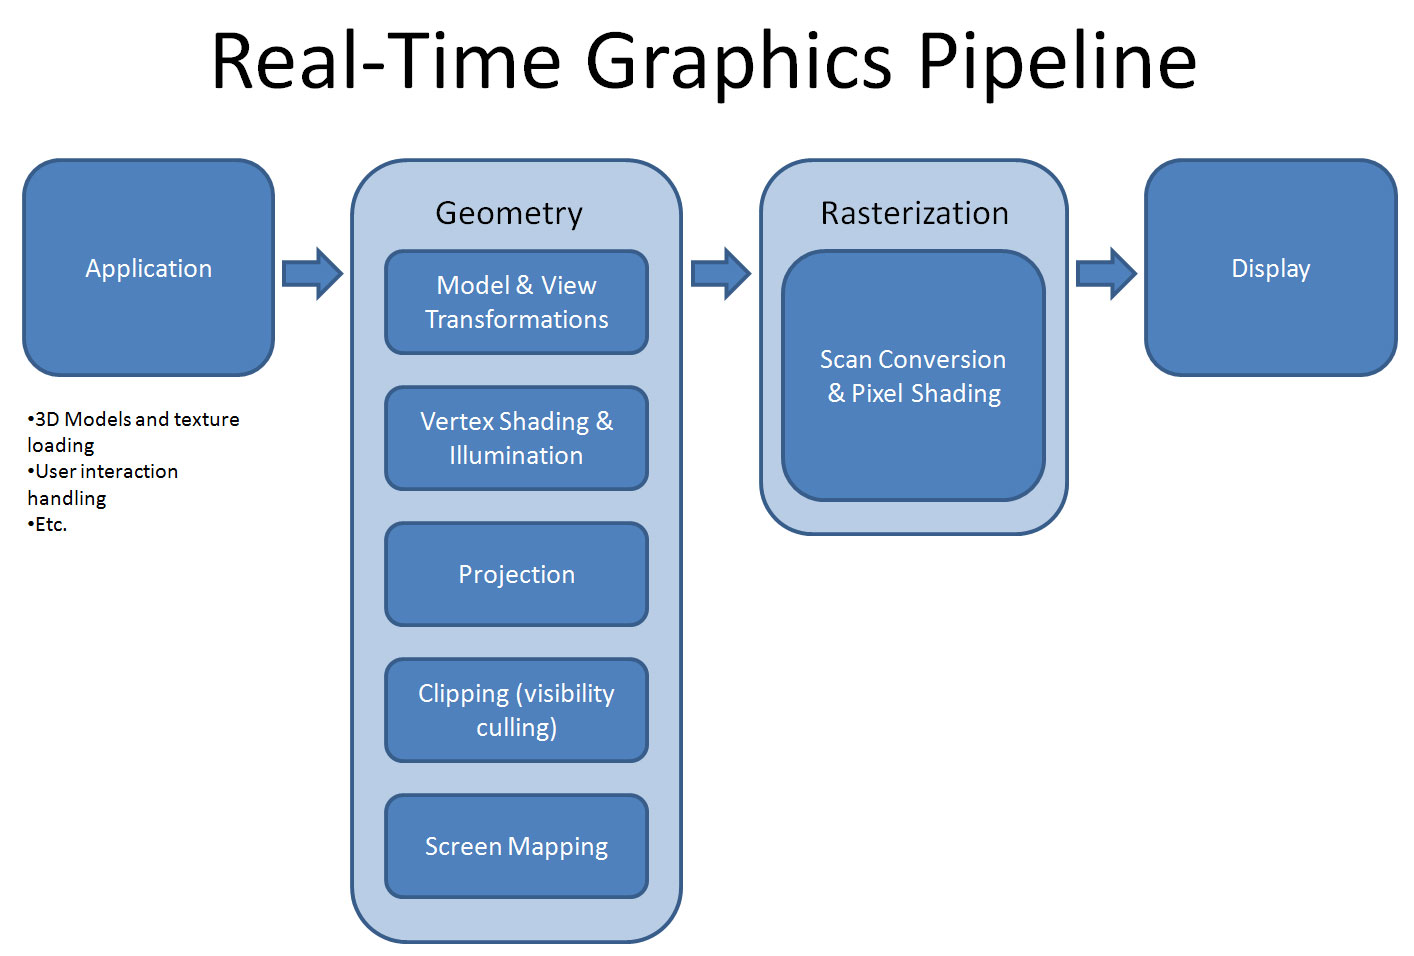
\includegraphics[width =.8\textwidth]{../figuras/renderingpipeline}
    \par\medskip
    Adaptado de: <http://www.cgchannel.com/2010/11/cg-science-for-artists-part-2-the-real-time-rendering-pipeline/>. 
    Acesso em: 27/05/2017.
    \label{renderingpipelinerep}
\end{figure}

\subsection{Aplicação}

A primeira etapa, a de aplicação, é executada na CPU\@. Esta é a parte a qual o 
desenvolvedor possui total controle, e na qual a maior parte das otimizações podem ser 
feitas para a melhora do desempenho do pipeline. 

Alguns exemplos de computações que são feitas nesse estágio são: gerenciamento de \textit{inputs}, 
detecção de colisão, animações de texturas, animações através de transformações, ajuste 
de parâmetros que são utilizados nas outras etapas, etc. Ao final dessa fase, toda a 
geometria e parâmetros computados são passados à fase de geometria.\ essa passagem de 
dados é considerado o passo mais importante da parte de aplicação.

\subsection{Geometria}

Na etapa de geometria a maior parte das operações sobre vértices e polígonos são feitas. 
Essa etapa ainda é subdividida em outras etapas menores: transformação de modelo e de 
visualização, \textit{vertex shading}, projeção, truncamento e mapeamento para tela. 
A transformação de modelo e de visualização converte o sistema de coordenadas de um 
vértice para coordenadas do mundo e coordenadas de visualização, respectivamente.

O \textit{vertex shading} é o processo pelo qual todos os vértices da cena passam e nessa 
parte serão definidas suas cores, posições, texturas, quantidade de iluminação e outros 
atributos. Todos esses atributos são então enviados para a etapa de rasterização onde 
serão interpolados.

Na etapa de projeção, ocorre uma transformação do volume de visualização, e o seu formato 
dependerá do tipo de projeção utilizada, alterando a percepção dos objetos da cena. 
A projeção utilizada neste trabalho 
é a projeção perspectiva, que transforma o volume de visualização em uma pirâmide 
truncada, chamada de \textit{frustum} de visualização, na qual os objetos mais próximos 
da base da pirâmide aparentam ser menores.

A etapa de truncamento serve para truncar os objetos da cena que estão sendo parcialmente 
vistos no volume de visualização. Objetos que possuem alguns vértices dentro e outros 
fora do volume de visualização precisam ter seus vértices que estão fora realocados para 
os extremos do volume de visualização.

Na última sub-etapa, a de mapeamento para tela, as coordenadas das primitivas truncadas 
dentro do volume de visualização são transformadas para a tela. As coordenadas $x$ e 
$y$ de cada primitiva são transformadas para formar as coordenadas da tela. As coordenadas 
de tela combinadas com as coordenadas $z$ são chamadas de coordenadas de janela. É nessa 
etapa que as coordenadas são essencialmente convertidas de tridimensionais para 
bidimensionais.

\subsection{Rasterização}

Com todos os dados para o devido \textit{shading} do objeto, nessa etapa as cores dos 
pixels são computadas e definidas, esse é o processo conhecido como rasterização, que é 
a conversão dos vértices em coordenadas de janela juntamente com a informação de 
\textit{shading} para pixels desenhados na tela.
Assim como a etapa de geometria, a etapa de rasterização também é dividida em sub-etapas, 
que são: configuração dos triângulos, \textit{triangle traversal}, \textit{pixel shading} 
e combinação. A seguir as etapas serão apresentadas conforme descrito 
por~\cite{akenine2008real}.

Na etapa de configuração dos triângulos, os dados sobre as superfícies dos triângulos 
são computados. Esses dados são utilizados para a interpolação de várias informações 
de \textit{shading} produzida na etapa de geometria, essa etapa de configuração dos 
triângulos é feita automaticamente pela GPU, não havendo opção de parametrização por 
parte do desenvolvedor.

Na etapa de \textit{triangle traversal} são procurados os pixels que estão dentro de 
um triângulo, ou seja, que pertencem ao plano formado pelos três vértices de um dos 
triângulos presentes na tela. Para cada um dos pixels encontrados é gerado um 
fragmento. As propriedades dos fragmentos de cada triângulo são geradas utilizando 
dados interpolados entre os três vértices.

No \textit{pixel shading}, são feitas todas as computações de \textit{shading} pixel 
por pixel, usando os dados interpolados como \textit{input}, resultando em uma ou mais cores 
para serem passadas à próxima etapa. Esta etapa, ao contrário das outras que são 
feitas por funções fixas do hardware dedicado, é feita por núcleos programáveis da 
GPU, nomeadamente pelo \textit{fragment shader}. Esse shader será responsável por 
aplicar texturas, iluminação, entre outros em cada um dos fragmentos.

Por fim, na combinação a informação de cada pixel é armazenada em um \textit{buffer} 
de cores, que contém cada um dos componentes RGB da cor final. A unidade da GPU 
responsável por essa etapa não é completamente programável, porém altamente 
customizável.
A cor resultante da etapa anterior (\textit{pixel shading}) é combinada com a cor 
atualmente armazenada no \textit{buffer}.

Essa etapa também é responsável por resolver a visibilidade, ou seja, armazenar no 
\textit{buffer} de cores somente as cores das primitivas que estão visíveis a partir 
do ponto de vista da câmera. Para a maior parte dos hardwares gráficos, isso é feito com 
o algoritmo do \textit{Z-buffer}. Esse algoritmo foi originalmente proposto por Edwin 
Catmull~\cite{Catmull1974}, seu funcionamento consiste no uso de um \textit{buffer} de 
profundidade, disposto em uma matriz bidimensional que armazena a profundidade de cada 
um dos pixels da tela. Quando um objeto precisa ser renderizado em um pixel já 
utilizado, o método compara as duas profundidades e caso o novo objeto esteja mais 
próximo do observador, o pixel é então sobrescrito por este objeto e o novo valor de 
profundidade substitui o antigo no \textit{buffer}.

Todos os \textit{buffers} combinados formam o chamado \textit{frame buffer}, que em 
consequência contém toda a informação de um quadro de uma cena renderizada. A tela exibe 
os conteúdos do \textit{buffer} de cores.

\section{O \textit{Loop} de Jogo}
\label{gameloopsec}

O \textit{loop} do jogo é onde os componentes funcionam em conjunto para proporcionar o que 
define um jogo: uma aplicação interativa em tempo real. 
Sistemas interativos em tempo real podem ser divididos em três módulos principais: 
recebimento de \textit{inputs}, processamento e apresentação dos 
resultados~\cite{dalmau2004core}.

Jogos possuem restrições de tempo para realizar todas as 
suas rotinas, se o sistema não for capaz de fazer seu trabalho dentro do limite de 
tempo irá falhar. Uma vez que sistemas interativos devem fazer suas tarefas 
em tempo real. Se um jogo não for capaz de fazer isso, o usuário (nesse caso o 
jogador) não receberá um \textit{feedback} contínuo, e o jogo não fornecerá a 
interatividade que deveria. Um \textit{loop} de jogo pode ser implementado com a 
finalidade de satisfazer essas restrições~\cite{Joselli2010}.

Nos jogos eletrônicos, o sistema de \textit{inputs} corresponde ao gerenciamento do dispositivo 
de entrada, como mouse, teclado ou controle de jogo; o processamento é responsável 
por tomar as decisões que afetam o estado do jogo, e a apresentação é responsável por 
mostrar os resultados desses dois outros estágios, através de áudio e 
vídeo~\cite{valente2005real}. 

Elaborar um \textit{loop} de jogo significa organizar esses três módulos, e seus submódulos na 
ordem apropriada para deixar a simulação o mais fiel o possível da experiência desejada. 
Considerando os módulos citados, o \textit{loop} do jogo pode ser dividido da seguinte 
maneira:
\begin{itemize}
    \item Detecção e gerenciamento de \textit{inputs}
    \item Estágio de processamento
    \item Estágio de apresentação
\end{itemize}

O estágio de processamento é ainda subdividido em outras partes, onde cada uma 
corresponde a um aspecto diferente do estado do jogo, como detecção de colisões, 
simulações físicas, a IA do jogo, aplicações das regras do jogo, etc. Estas portanto, 
também devem ser organizadas na ordem correta. No estágio de apresentação são 
reproduzidos todos os áudios necessários e a cena é renderizada na tela com os 
resultados dos estágios anteriores.

Uma medida de desempenho de aplicações gráficas que também é utilizada para medir a 
frequência com a qual esses \textit{loops} são executados é a quantidade de quadros por 
segundo (\textit{Frames per Second}) que são renderizados na tela, conhecido como 
FPS. Cada quadro que aparece na tela representa uma imagem construída e apresentada 
pela aplicação.

O desempenho de um jogo, além de ser dependente das otimizações feitas a nível de 
software, é também dependente da configuração de hardware da plataforma na qual será 
executado. Portanto, um mesmo jogo pode rodar com um FPS diferente dependendo da 
plataforma utilizada, visto que a atualização do estado do jogo é dependente da 
quantidade de quadros construídos, uma mesma sequência de eventos pode ter um 
resultado diferente dependendo do poder computacional do hardware. 

Para evitar esse problema, é necessário tornar o estágio de processamento independente 
da taxa de FPS. Isso pode ser feito adicionando um parâmetro de tempo ao estágio de 
processamento. Esse parâmetro corresponde ao tempo decorrido entre a atualização 
atual e a última atualização do processamento feita~\cite{valente2005real}, e é 
conhecido como \textit{delta time}, indicando uma diferença de tempo.

Além da separação do estágio de processamento em sub-tarefas, é importante salientar 
que nem todas possuem a mesma necessidade de atualização que outras. Por exemplo, a IA 
não precisa ser atualizada com a mesma frequência que a simulação física, 
é necessário somente quando um agente precisa tomar uma decisão. A renderização por 
outro lado, proporcionará um resultado melhor quanto mais atualizada esta for, desde 
que não comprometa o desempenho geral do sistema. Por isso, uma forma de otimizar o 
desempenho é atualizar cada um dos componentes somente quando necessário.

\section{Interpolações}

Na seção~\ref{gameloopsec}, foi discutido o problema da atualização do estado do jogo em 
relação à taxa de quadros por segundo com a qual a aplicação está sendo executada, e 
como esse problema pode ser solucionado adicionando um parâmetro que indica o tempo 
decorrido entre o último quadro e o atual.

Interpolação é um dos recursos utilizados na solução deste problema, e é utilizada para 
qualquer caso em que se queira passar uma noção de locomoção ou movimento entre os 
diversos quadros, seja através de animações, aplicação de forças, rotações, etc.

Caso se queira adicionar um vetor de velocidade a um objeto, esse objeto passará a ter 
duas velocidades: a velocidade inicial, a qual ele já possui, e a velocidade alvo, a qual 
é uma combinação de sua velocidade inicial com a nova velocidade aplicada. Se a alteração 
da velocidade inicial para a velocidade alvo fosse feita de um quadro para o outro, o 
objeto teria uma aceleração instantânea (ou desaceleração) completamente não natural e 
não realista. A interpolação serve para calcular os pontos intermediários entre esses 
dois extremos a partir de um parâmetro que determinará quantos pontos intermediários 
serão gerados. No exemplo da velocidade, esse parâmetro pode ser uma combinação entre 
uma aceleração e o tempo decorrido entre um quadro e outro (\textit{delta time}). Dessa 
maneira, a alteração da velocidade será feita de uma maneira gradual e independente da 
taxa de quadros por segundo.

A classe geral de funções utilizadas para interpolações são chamadas de curvas 
paramétricas. Dado os dois pontos sendo interpolados, uma interpolação entre estes 
pode ser entendida como uma curva formada entre suas posições, onde o parâmetro 
supracitado determinará em que posição se está nessa curva. O exemplo mais simples de uma 
curva paramétrica é dado por:

\begin{equation}
    \begin{aligned}
        L(t) = (1 - t \cdotp P_0 + t \cdotp P_1
    \end{aligned}
\end{equation}

\vspace{1cm}

Esta é uma interpolação linear, onde $L(t)$ é um ponto intermediário, $P_0$ é o ponto 
inicial, $P_1$ é o ponto alvo e $t$ é o parâmetro utilizado para controlar a posição em 
que se está na linha relativa a $P_0$ e $P_1$. Nota-se que $t$ varia em um intervalo 
entre $[0,1]$, quanto mais próximo de $0$, mais próximo de $P_0\ $ se estará e quanto 
mais próximo de $1$ mais próximo de $P_1\ $ se estará. 

Esse conceito de interpolação linear pode ser estendida para vetores e quaternions por 
exemplo, permitindo a aplicação gradual de forças e de rotações.
Na área de Computação Gráfica, é popular a utilização do jargão "lerp"\ para se referir 
à interpolação linear, uma abreviação de \textit{Linear Interpolation}.

\subsection{Interpolação Entre Vetores}

A interpolação linear entre dois vetores é semelhante à interpolação entre dois pontos 
vista anteriormente. A diferença é que o cálculo da interpolação é feito componente a 
componente, semelhante às outras operações entre dois vetores:

\begin{equation}
    \begin{aligned}
        Lerp(u,v,t) = ((1 - t) \cdotp u_x + t \cdotp v_x, \\
                      (1 - t) \cdotp u_y + t \cdotp v_y, \\
                      (1 - t) \cdotp u_z + t \cdotp v_z)
    \end{aligned}
\end{equation}

\vspace{1cm}

\subsection{Interpolação Entre Quaternions}

Para interpolar dois quaternions, é necessário calcular o menor caminho do ângulo formado 
entre os dois, visto$\ $ que a interpolação é feita de maneira circular. Para realizar este 
cálculo, utiliza-se o produto escalar entre os dois quaternions, que retornará o cosseno 
do ângulo e dependendo do seu valor, parâmetros diferentes são utilizados:

\begin{equation}
    \begin{aligned}
        \cos \theta = q_1 \cdotp q_2 \\
        t_1 = 1 - t \\
        q_i = 
        \begin{cases}
            (q_1 \cdotp t_1) + (q_2 \cdotp t) & \quad \text{se } \cos \theta > 0 \\
            (q_1 \cdotp t_1) + (q_2 \cdotp -t) & \quad \text{se } \cos \theta < 0 \\
        \end{cases}
    \end{aligned}
\end{equation}

\vspace{1cm}

Onde $q_1$ e $q_2$ são os dois quaternions sendo interpolados, $t$ é o parâmetro de 
interpolação e $q_i$ é o quaternion resultante da interpolação. É importante ressaltar 
que $q_i$ deve ser normalizado ao final da interpolação.

Quaternions ainda possuem um outro tipo de interpolação, a interpolação linear esférica, 
que é um pouco mais custosa de se calcular do que a interpolação linear normal, porém 
possui uma precisão maior. Essa interpolação é conhecida como "slerp", abreviação de 
\textit{Spherical Linear Interpolation}. Utilizando os mesmos parâmetros da outra 
interpolação, a slerp é dada por:

\begin{equation}
    \begin{aligned}
        \theta = \arccos(q_1 \cdotp q_2) \\
        t_1 = \sin((1 - t) \cdotp \theta / \sin \theta) \\
        t_2 = \sin(t \cdotp \theta / \sin \theta) \\
        q_i = (t_1 \cdotp q_1) + (t_2 \cdotp q_2)
    \end{aligned}
\end{equation}

\vspace{1cm}

Assim como na interpolação linear normal, aqui $q_i$ também deve ser normalizado ao final 
da operação.

\section{Considerações Finais do Capítulo}

Neste capítulo foram apresentados os fundamentos utilizados para o desenvolvimento do 
trabalho proposto, que possui um alto fator interdisciplinar.
A modelagem orientada a dados é um termo que surgiu recentemente, porém seu conceito de 
uso eficiente e sequencial da memória já é utilizado a mais tempo. Foram apresentados 
alguns de seus principais princípios, suas diferenças com a programação orientada a 
objetos, que atualmente é considerada o padrão na indústria, e como a restruturação de 
código utilizando essa abordagem pode proporcionar uma melhora no desempenho de uma 
aplicação.

Os motores de jogos revolucionaram o modo como os jogos são feitos na indústria através 
da clara separação entre o conteúdo técnico e o criativo de um jogo. Foi explicado o 
surgimento deste conceito, a filosofia de implementação de um motor de jogo, a 
importância da integração apropriada de seus componentes e também foram apresentados 
alguns exemplos de componentes comuns em motores de jogos.

Foram apresentados os \textit{pipelines} de visualização e renderização, dois 
conceitos importantes em aplicações gráficas que consistem em etapas que processam os 
dados desde o seu carregamento no sistema até serem transformados em pixels na tela, 
e como o renderizador gráfico de baixo nível auxilia nas etapas da renderização.
Outros conceitos importantes de Computação Gráfica também foram explicados, como 
\textit{shaders}, iluminação e malhas de polígono.

Foi apresentado o conceito do \textit{loop} de jogo,
encarregado de receber e gerenciar os \textit{inputs} do jogador, atualizar os 
componentes que necessitam fazê-lo, e apresentar os resultados computados.
Também foi discutido sobre alguns de seus problemas, como a necessidade de diferentes 
frequências de atualização de cada um dos componentes, e também como os resultados 
das atualizações podem ser diferentes dependendo do poder computacional do hardware 
utilizado. Foi apresentada uma solução para este problema, e também uma medida de 
desempenho popular para jogos, a taxa de quadros por segundo (FPS).

Por fim, foi apresentado o conceito de interpolações e como o seu uso se relaciona com 
o problema da variação de FPS em jogos. Além disso, foram apresentados exemplos de 
implementação da interpolação linear para vetores e quaternions.

\chapter{Trabalhos Relacionados}
\label{relatedworkscap}

Neste capítulo serão apresentados alguns trabalhos encontrados na literatura que estão relacionados 
com a proposta deste trabalho. A maioria dos trabalhos apresentados concentra-se em criar 
funcionalidades únicas para um motor de jogos e também nas melhores práticas para o 
desenvolvimento de motores de jogos, porém nenhum destes trabalhos explora o uso da 
modelagem orientada a dados.
Apesar de nenhum deles estar diretamente relacionado com a proposta deste trabalho, os 
autores também tinham como um dos objetivos desenvolver um motor de jogos eficiente e 
bem estruturado.

O trabalho de Freitas~\cite{deFreitas2012GEC} propôs um modelo de motor de jogos com uma 
arquitetura baseada em componentes, na qual as entidades do jogo são definidas através 
da agregação de componentes, em contraste com os modelos clássicos os quais utilizam 
hierarquia de classes e heranças múltiplas, que leva a problemas como forte 
interdependência das entidades, conflito de nomenclaturas e heranças repetidas.

Esta arquitetura baseada em componentes atualmente é utilizada em motores de jogos 
comerciais populares, como é o caso do motor de jogos de propósito geral 
Unity3D\footnote{Site do Unity3D: https://unity3d.com}. Nesse 
modelo, uma entidade pode ter características diferentes adicionadas a ela através da 
adição de componentes configuráveis, como um componente renderizador de imagens, um 
reprodutor de áudios, um corpo suscetível à aplicação de forças físicas, entre outros. 
Este modelo de arquitetura permite então a criação de entidades com uma maior 
flexibilidade, adaptabilidade e independência, além de não apresentar os problemas do 
uso de herança.

O trabalho deles prossegue então, para explicar seus diferenciais, como a utilização de 
entidades que permitem a sua reconfiguração dinâmica em diferentes 
momentos da aplicação. Consequentemente isso permite flexibilidade e extensibilidade 
até mesmo em tempo de execução. Por fim eles apresentam as decisões de design que os 
permitiram atingir esses objetivos.

\citeonline{Anderson2008} discute em seu trabalho alguns problemas ainda pendentes 
em se tratando de desenvolvimento de motores de jogos, e incentiva a pesquisa no campo 
de arquitetura e design de motores de jogos. 

Primeiramente, os autores comentam sobre o aumento significativo do uso motores de 
jogos, pela produtividade de desenvolvimento que estes proporcionam. Depois é mencionada a falta 
de literatura e pesquisa a respeito de modelagem e arquitetura de motores de jogos em 
geral, sendo que a maioria do material encontrado tem ênfase apenas na implementação dos 
componentes individuais, enquanto que as estratégias utilizadas para a modelagem dos 
motores como um todo não são comentadas, sendo então difícil encontrar material que 
apresente uma explicação minuciosa sobre a modelagem e estruturação da arquitetura de 
um motor de jogos.

Depois dessa introdução, são mencionados alguns problemas persistentes nessa área, que 
podem ser potenciais áreas de pesquisa a respeito de motores de jogos. O primeiro 
problema e que há uma falta de convenção sobre as terminologias utilizadas em desenvolvimento de 
jogos, frequentemente levando a problemas de comunicação e pesquisa eficiente e confusão 
entre os estudantes novos na área. 

O segundo problema mencionado é a dificuldade na determinação do limite entre o que faz 
parte do jogo propriamente dito e o que faz parte do motor de jogos. Não há uma 
definição concreta sobre o que é um motor de jogos e existem várias versões diferentes, 
frequentemente levando ao equívoco no entendimento sobre o conceito de um motor de 
jogos. 

O terceiro problema mencionado é sobre as decisões de modelagem do motor de jogos, e 
como diferentes gêneros de jogos afetam essas decisões, pois algumas estratégias em 
específico beneficiam somente uma certa classe de jogos. É levantada então a 
questão da possibilidade de definição de um motor de jogos que é eficiente para qualquer 
jogo independente do seu tipo.

O quarto problema mencionado é sobre o impacto que as rotinas de baixo-nível dos motores 
de jogos causam na modelagem de alto-nível do mesmo, comentando sobre a constante 
evolução da tecnologia utilizada em dispositivos de hardware ou nas interfaces do 
software e suas capacidades, e como essas mudanças podem afetar a evolução de um ou 
múltiplos componentes do motor de jogos.

O último problema mencionado é sobre as melhores convenções e práticas de programação 
que devem ser utilizadas na modelagem de um motor de jogos. Como os motores de jogos 
estão em constante crescimento e evolução desde seus desenvolvimentos iniciais, a 
adição de novas funcionalidades pode ser problemática ou até mesmo impossível, se os 
objetivos no motor de jogos não foram bem definidos no início do projeto, ou se sua 
arquitetura não foi bem estruturada. Os autores ponderam então se existe um conjunto de 
melhores práticas para evitar ou reduzir estes problemas.

\citeonline{Keenan2011} salientam a importância da definição de uma boa arquitetura para 
o desenvolvimento de um motor de jogos. Em seu trabalho, ele menciona os problemas 
relacionados com a má estruturação do motor de jogos, e como a criação de um sistema 
flexível e modularizado pode evitar esses problemas, além de proporcionar outras 
vantagens.
Como o seu trabalho é para fins educativos, o restante do artigo trata sobre a 
criação de um curso sobre arquitetura de jogos, no qual o foco não é a implementação dos 
componentes separados do motor de jogos, mas sim a utilização das melhores práticas de 
programação e modelagem para a construção de um motor de jogos com uma arquitetura 
robusta.

\citeonline{Zhu2016ECG} propõem uma nova metodologia para o desenvolvimento de jogos, 
chamada de \textit{Engine- Cooperative Game Modeling} (ECGM), um modelo híbrido 
que combina duas outras metodologias: \textit{Model-Driven Game Development} (MDGD) e a 
cadeia de ferramentas do motor de jogos, com ênfase nos aspectos técnicos. A motivação 
de seu trabalho é que nenhuma das abordagens para o MDGD na literatura demonstrou 
convincentemente uma boa integração do MDGD com a cadeia de ferramentas do motor de 
jogos.
No restante do trabalho, é descrito o funcionamento desta metodologia proposta, e como 
ela pode fornecer uma melhoria na modelagem dos projetos ao utilizar o MDGD levando em 
consideração a cadeia de ferramentas tipicamente utilizadas em motores de jogos.

Um trabalho mais relacionado ao tema modelagem orientada a dados é o proposto 
por~\citeonline{Fontana2017}, no qual o DOD é utilizada no desenvolvimento de uma 
ferramenta \textit{opensource} de projeto físico de circuitos integrados. No trabalho 
são discutidos os principais conceitos do DOD, como esta pode ser utilizada para aprimorar 
a qualidade do \textit{software} e como pode ser utilizada no contexto de problemas de 
projeto físico, que assim como jogos, também precisa lidar com uma substancial quantidade 
de dados.

Para validar os fundamentos discutidos, foi desenvolvido um sistema utilizando um padrão de 
projeto conhecido como modelo entidade-componente, que consiste em decompor um problema 
em um conjunto de entidades e seus componentes (chamados de propriedades). Os resultados 
obtidos foram comparados com um outro sistema com uma abordagem orientada a objetos para 
testar o desempenho do sistema com DOD.\@ As métricas escolhidas foram o tempo de execução e 
a quantidade de \textit{cache misses} para dois problemas diferentes. 

Os resultados obtidos pelos autores mostram que um problema em um cenário com boa 
localidade de dados, isto é, cenários que requerem poucas propriedades de cada entidade, o 
DOD é cerca de 90\% mais rápida que a orientação a objetos. Enquanto que em um cenário com 
uma má localidade de dados, que requer o acesso a uma quantidade superior de propriedades 
diferentes das diferentes entidades do sistema, o DOD apresenta um desempenho apenas 6\% 
pior em média.

\section{Considerações Finais do Capítulo}

Dados os problemas mencionados nos trabalhos relacionados, percebe-se que a maior 
dificuldade no desenvolvimento de um motor de jogos não consiste na implementação dos 
componentes individuais que compõem o motor, mas sim na integração adequada destes 
componentes e no projeto e modelagem eficientes do motor. 

Como foi mencionado, a maior parte do material encontrado concentra-se na implementação 
dos componentes individuais e nas otimizações feitas sobre estes, como por exemplo as 
otimizações que podem ser feitas em algoritmos de inteligência artificial comumente 
utilizados em jogos. Como a proposta deste trabalho se concentra exatamente em uma 
abordagem diferente para a modelagem e estruturação dos componentes do motor de jogos 
e consequentemente na integração destes, foi possível encontrar trabalhos apenas 
parcialmente relacionados.

Além disso nenhum dos trabalhos encontrados deu ênfase nos problemas que podem surgir 
do uso da programação orientada a objetos em jogos, e quais são as alternativas ou 
práticas que podem contornar esses problemas. Apesar de alguns trabalhos mencionarem 
maneiras de melhorar a arquitetura e projeto de um motor de jogos, ou proporcionar 
uma maior flexibilidade e extensibilidade, nenhum deles discute sobre como melhorar a 
estrutura desses componentes, principalmente levando em consideração a evolução do 
hardware, conforme mencionado por Anderson~\cite{Anderson2008}.

\chapter{Otimizações para motores de jogos através de modelagem 
orientada a dados}
\label{proposalcap}

Para testar as otimizações proporcionadas pela modelagem orientada 
a dados, um motor de jogos foi desenvolvido em duas versões 
diferentes: uma utilizando os conceitos da programação orientada a 
objetos, e outra utilizando modelagem orientada a dados,
visando à otimização da comunicação entre o processador e a memória.
A versão com abordagem de programação orientada a objetos será 
referida como primeira versão, ou versão OO (orientada a objetos). A 
outra versão com a abordagem de modelagem orientada a dados será referida 
como segunda versão, ou versão OD (orientada a dados).
Além de utilizar os conceitos do DOD, também é necessário 
utilizar conceitos de Computação Gráfica, Álgebra Linear e Geometria Analítica, Teoria 
de Grafos, Processamento de Imagens, Física, entre outros.

Conforme explicado na seção~\ref{secgameengine}, um motor de jogos é uma combinação de 
diversos componentes diferentes que compõem a parte lógica de um jogo digital. As 
seções seguintes discutirão sobre os componentes implementados que foram julgados 
necessários para o desenvolvimento do motor de jogos que é o objeto de estudo deste 
trabalho, bem como as diferenças entre as implementações.

Além dos componentes, também serão explicadas as estratégias empregadas para a 
implementação de outros elementos importantes discutidos previamente no 
capítulo~\ref{theorycap} que fazem parte da estrutura de um motor de jogos, como o 
\textit{pipeline} de renderização e o loop de jogo.

Como um motor de jogos por si só não é suficiente para se gerar análises e resultados,
além do desenvolvimento do motor, foi necessário o desenvolvimento de dois cenários 
diferentes em ambas as versões do motor que utilizasse as suas funcionalidades e 
verificar a sua eficiência nos diferentes casos. As aplicações desenvolvidas 
são idênticas para as duas versões do motor. O primeiro cenário possui um bom padrão 
de acesso à memória para a verão orientada a objetos e um mal padrão de acesso para a 
versão orientada a dados, o segundo cenário é o inverso. Mais detalhes a respeito dos 
dois cenários desenvolvidos serão explicados no capítulo~\ref{resultscap}.

A análise de desempenho das principais funções da aplicação 
permitirá a comparação entre as duas abordagens e a eficiência do
DOD. Além das alterações necessárias nos componentes do motor, há 
também alterações a serem feitas na aplicação de teste 
desenvolvida, estas serão apresentadas para demonstrar a conversão 
entre as abordagens. Apesar das diferenças, nem todos os componentes 
sofreram alterações entre as duas versões, por este motivo não 
serão apresentadas alterações para todos os componentes descritos 
nesse capítulo.

A figura~\ref{umlengine} contém um diagrama de classes com as principais
classes do motor e as relações entre estas na versão orientada a objetos. Os 
componentes do motor juntos contém o mínimo necessário para executar uma 
aplicação gráfica 3D utilizando openGL. O componente gráfico é composto pelas 
classes ProgramaShader, GrafoCena, NoGrafo, Camera e Malha. O componente da 
física é composto pela classe Objeto. 

\begin{figure}[h!]
    \centering
    \captionof{figure}{UML simplificado contendo os principais componentes do motor.}
    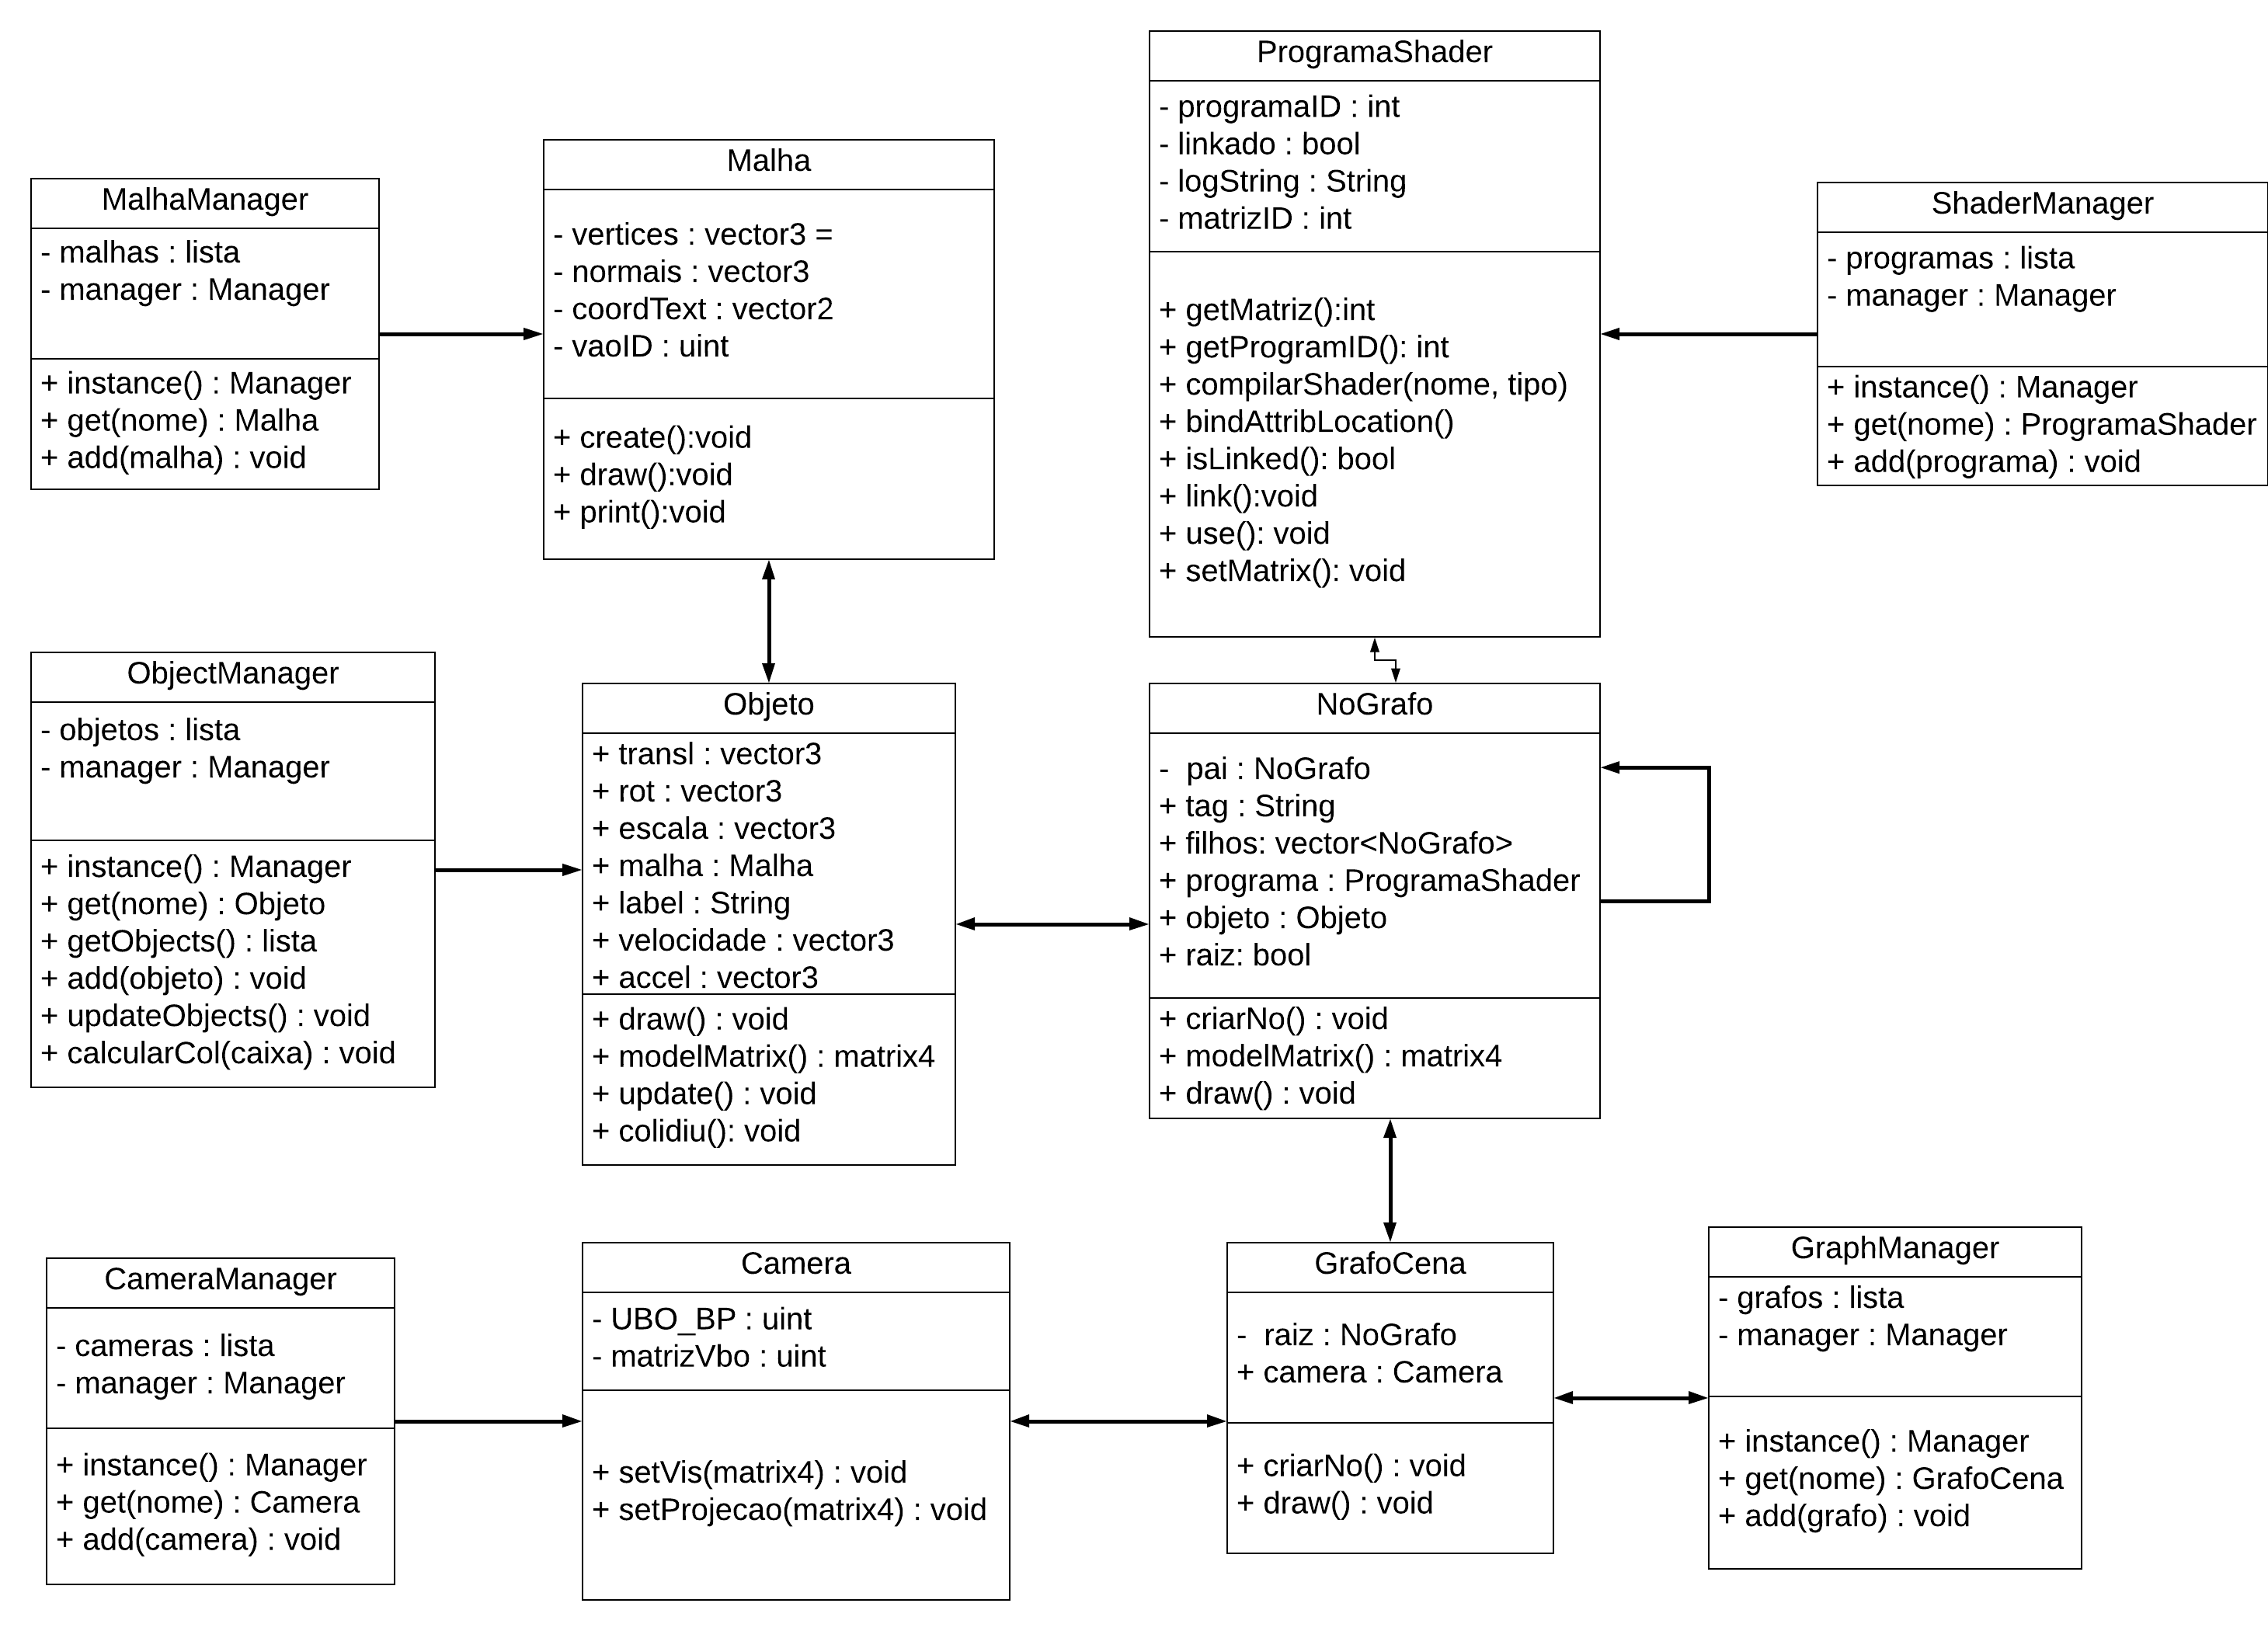
\includegraphics[width =.8\textwidth]{../figuras/uml_engine}
    \par\medskip
    Fonte: autoria própria
    \label{umlengine}
\end{figure}

Para o gerenciador de recursos foi 
utilizado o padrão de \textit{singletons}, no qual as 
classes que são \textit{singletons} restringem a instanciação de objetos da 
classe para exatamente um. As classes do tipo Manager apresentadas na 
figura~\ref{umlengine} são \textit{singletons} que controlam o armazenamento e 
acesso aos principais recursos da aplicação, que são as malhas, objetos, grafos 
de cena, cameras e shaders.

O primeiro passo feito para realizar a conversão do motor para uma abordagem 
orientada a dados, conforme descrito na sessão~\ref{secdataorienteddesign}, 
foi analisar o fluxo de dados necessário para que cada um dos componentes 
funcionem apropriadamente, e especificar quais são os dados gerados 
por cada componente. Depois de determinar o fluxo, o próximo passo foi 
descrever as transformações de dados que cada componente precisa 
realizar.

Após analisar os componentes do motor e a aplicação desenvolvida, 
pode-se observar que o fluxo de dados ocorre na seguinte ordem:
\begin{enumerate}
    \item Os recursos externos são carregados no sistema (\textit{shaders} e malhas).
    \item Os objetos e o grafo de cena são criados e alocados.
    \item Inicia-se o ciclo principal do programa:
        \begin{enumerate}
           \item Atualização dos objetos.
           \item Verificação de colisões.
           \item A câmera atualiza a matriz de visualização e projeção.
           \item O grafo de cena é renderizado.
        \end{enumerate}
\end{enumerate}

Com o fluxo de dados definido, é necessário analisar as 
transformações necessárias dos dados. A parte relevante do 
sistema a ser analisada é o ciclo principal, pois é a única parte 
do fluxo de dados que será executada em tempo real.

A primeira etapa do ciclo principal é a atualização dos objetos. 
Primeiramente a aceleração do objeto é atualizada através de 
fórmulas arbitrárias, posteriormente a velocidade é atualizada 
utilizando a aceleração. Com a velocidade atualizada a última 
parte é atualizar a translação e a rotação, ambas são atualizadas 
através da velocidade.

A segunda etapa é a verificação de colisões, isso é feito 
utilizando as dimensões de uma caixa retangular e o componente 
de translação do objeto. O procedimento de verificação de colisão 
simplesmente testa se o componente de translação do objeto não 
ultrapassa as bordas da caixa.

A terceira etapa consiste na atualização das matrizes de 
visualização e projeção da cena. A atualização ocorre somente uma 
vez por frame, e como há somente uma câmera na cena, essa etapa 
não possui muito potencial para otimização.

A última etapa é a renderização do grafo de cena. Para cada nó 
presente no grafo, essa etapa é 
dividida em três partes: cálculo das coordenadas do objeto, 
conversão dessas coordenadas para coordenadas do mundo, e a 
renderização do grafo.

O cálculo das coordenadas do objeto é feito 
através da multiplicação entre a translação, rotação e escala do 
objeto atribuído ao nó. A conversão das 
coordenadas do objeto para as coordenadas do mundo é feita utilizando 
as coordenadas do objeto e a hierarquia do grafo de cena. Por fim 
a última parte é a renderização propriamente dita, na qual não 
há processamento de dados, somente chamadas de métodos da API do 
openGL sobre dados já processados. Os dados necessários para a 
renderização de um nó são a malha atribuída ao objeto deste nó, 
o programa de shader atribuído ao nó e as coordenadas convertidas.

Com o fluxo de dados definido, assim como as transformações sobre 
os dados necessárias, é possível determinar quais são os dados 
mínimos necessários para a execução de aplicação e como 
agrupá-los.

Seguindo a premissa do DOD de descrever as transformações de 
dados sempre para o caso mais provável, as estruturas de dados 
utilizadas para o motor na versão orientada a dados foram 
feitas considerando que em uma aplicação sempre haverá 
várias instâncias de \textit{shaders}, malhas, objetos 
e nós do grafo de cena.

\begin{figure}[h]
    \centering
    \captionof{figure}{Estruturas utilizadas na verão orientada a dados do motor.}
    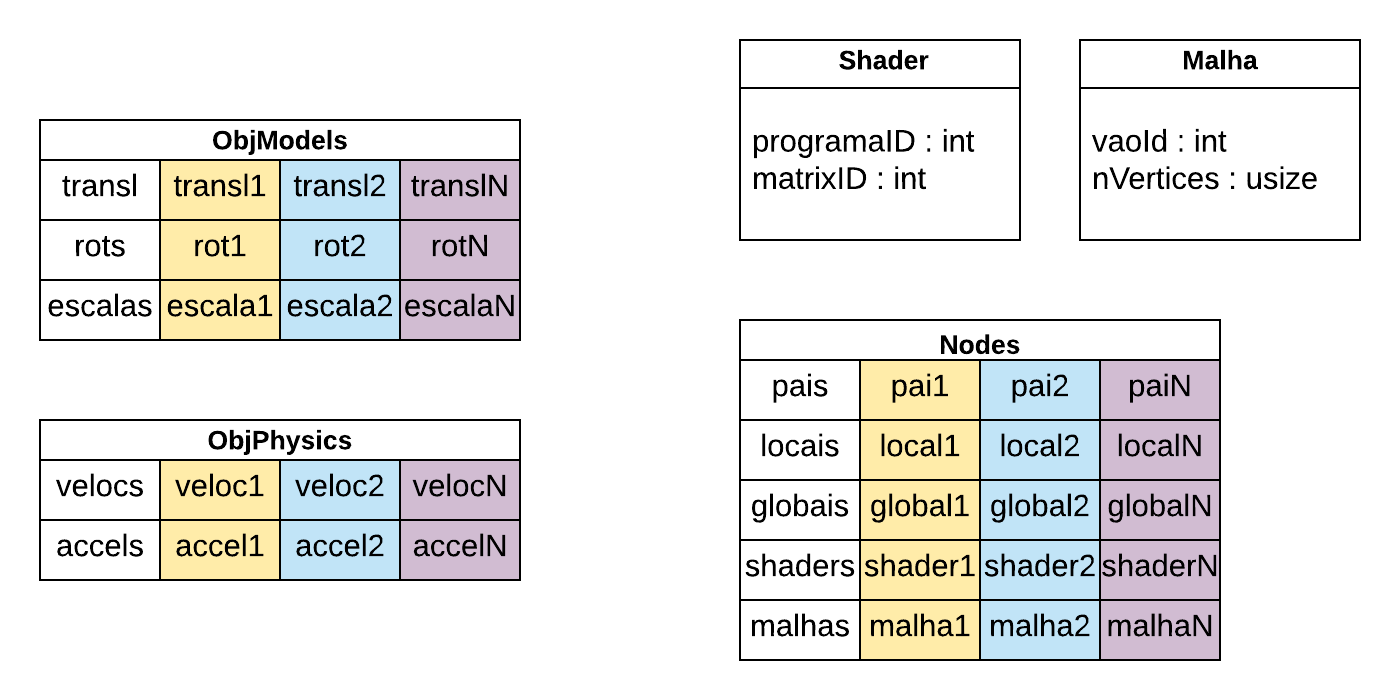
\includegraphics[width =.8\textwidth]{../figuras/dodengine}
    \par\medskip
    Fonte: autoria própria
    \label{dodengine}
\end{figure}

A figura~\ref{dodengine} apresenta as estruturas utilizadas no ciclo principal de 
execução da aplicação com uma abordagem orientada a dados, utilizando o layout SoA 
discutido na seção~\ref{secdataorienteddesign}. As classes de programa de 
shader e malha foram separadas em duas partes: interfaces para a criação de shaders 
e malhas a partir de arquivos externos, e estruturas simples contendo somente dados 
primitivos utilizados no ciclo principal. As estruturas de nós e objetos possuem 
\textit{containers} de $N$ elementos para os atributos principais das respectivas 
classes da versão orientada a objetos. A classe de objeto foi dividida em duas 
estruturas: uma para os dados da matriz de transformação (translação, rotação e 
escala), e a outra para dados de física (velocidade e aceleração).

Cada entidade no sistema possui seu identificador único representado 
por um número inteiro positivo e seus atributos são espalhados pelas estruturas 
que contém \textit{containers}. Ou seja, a referência ao item $0$ 
de qualquer um dos \textit{containers} apresentados na 
figura~\ref{dodengine} refere-se à mesma entidade. Através desse 
ID único de uma entidade os componentes são capazes de transformar 
e mover os dados entre si.

A seguir serão descritos com detalhes os componentes um a um 
presentes nos motores implementados. Para os componentes que 
possuem diferenças de implementação entre as duas versões também 
serão discutidas quais foram as mudanças necessárias para o 
desenvolvimento da versão orientada a dados.

\section{Biblioteca Matemática}

Utilizando os conceitos discutidos na seção~\ref{secmathconcepts}, foi 
desenvolvido uma biblioteca matemática o mais minimalista o possível, contendo somente 
as estruturas e funções necessárias para se realizar os testes e obter os resultados 
desejados deste trabalho. 

A biblioteca é uma das partes do motor mais extensivamente utilizada pois uma 
considerável parcela dos componentes necessitam dela. Além disso, todas as 
malhas e outros dados que são enviados aos \textit{shaders} programáveis são armazenados em 
estruturas dessa biblioteca, como as matrizes de transformação, visualização e projeção, 
fontes de luz, texturas, etc.

A biblioteca possui três estruturas: vetores, matrizes e quaternions. Para cada uma das 
estruturas há diversas funções diferentes associadas a elas. Além das funções associadas 
às estruturas, existem também funções e utilidades que não são inerentes a nenhuma delas, 
somente da biblioteca em si. 

Para todas as estruturas, o tipo das variáveis utilizadas são os números reais, mais 
especificamente, ponto flutuante de precisão simples. A precisão simples é a utilizada em 
jogos ou outras aplicações gráficas pois geralmente esse nível de precisão já é o 
suficiente, além de ter os benefícios de consumir menos memória e realizar operações 
aritméticas com mais eficiência do que pontos flutuantes de precisão 
dupla~\cite{Verth:2008}.

\subsection{Vetores}

Para os vetores, há uma estrutura separada para os vetores 3D e para os 4D. Os vetores 
2D não estarão presentes na biblioteca pois não terão uso para a aplicação pretendida.

Além do acesso individual a cada um dos componentes do vetor e sua manipulação direta, 
as seguintes funções são suportadas para vetores:
\begin{itemize}
    \item Operações aritméticas: adição e subtração entre vetores, multiplicação ou 
        divisão por escalar e igualdade entre vetores.
    \item Cálculo da magnitude de um vetor.
    \item Magnitude ao quadrado: essa função é similar à magnitude, com a diferença de 
        que essa função não calcula a raiz quadrada da soma dos quadrados dos 
        componentes. Caso a finalidade do cálculo da magnitude seja apenas para comparar 
        dois vetores, esse função já basta, e é mais eficiente pois poupa o cálculo 
        custoso da raiz quadrada.
    \item Normalização: existe duas funções diferentes, uma delas apenas normaliza o 
        vetor, enquanto a outra mantém o vetor inalterado e retorna a sua versão 
        normalizada.
    \item Produto escalar entre dois vetores.
    \item Produto vetorial entre dois vetores: essa função é exclusiva para vetores 
        3D.
    \item Interpolação linear entre dois vetores.
\end{itemize}

\subsection{Matrizes}

Assim como os vetores, as matrizes também possuem uma estrutura separada para matrizes 
$3 \times 3$ e $4 \times 4$, porém somente esses dois tipos de matrizes quadradas estão 
presentes pois são as únicas necessárias para a implementação da aplicação.

As matrizes possuem suporte à acesso individual a cada elemento e também a manipulação 
direta destes. Além disso, possuem as seguintes funcionalidades:
\begin{itemize}
    \item Adição, subtração e igualdade entre matrizes.
    \item Multiplicação por escalar.
    \item Cálculo da matriz transposta.
    \item Multiplicação entre matrizes.
    \item Multiplicação entre uma matriz e um vetor: essa função trata o vetor como uma 
        matriz linha ou matriz coluna, dependendo da ordem. Essa função requer uma 
        implementação diferente para cada uma das duas possibilidades de ordem dos 
        operandos.
    \item Cálculo da matriz inversa e do determinante da matriz: essas duas funções são 
        exclusivas para matrizes $3 \times 3$.
\end{itemize}

\subsection{Quaternions}

Só há uma estrutura para os quaternions, com acesso aos seus componentes escalar $t$, e 
ao vetorial $x,y,z$. Um quaternion pode ser construído tanto passando o valor dos seus 
quatro componentes, quanto passando um ângulo e um eixo, útil para se fazer uma 
transformação de rotação.

A estrutura de quaternion possui as seguintes funcionalidades associadas:
\begin{itemize}
    \item Adição, subtração e igualdade entre quaternions.
    \item Multiplicação por escalar.
    \item Multiplicação entre quaternions.
    \item Produto escalar entre quaternions.
    \item Extração do ângulo do quaternion.
    \item Extração do eixo do quaternion.
    \item Cálculo da norma.
    \item Normalização. Semelhante aos vetores, pode simplesmente normalizar ou retornar 
        uma cópia normalizada.
    \item Conversão para matriz.
    \item Interpolação linear e interpolação linear esférica entre quaternions.
\end{itemize}

\subsection{Outras Utilidades}

Além das funções mencionadas anteriormente, ainda existem algumas outras funções que 
servem como convenções para facilitar o processo de desenvolvimento e minimização de 
código escrito.

A biblioteca matemática também possui funções que não estão associadas com nenhuma 
estrutura, por exemplo, funções trigonométricas tais como: cotangente, conversão de 
graus para radianos e vice-versa.

Há constantes que também são utilizadas com frequência, como PI, epsilon, e um limitante 
arbitrário de pontos flutuantes. Esse limitante é utilizado para calcular a igualdade 
entre pontos flutuantes e consequentemente, todas as estruturas implementadas. Essa 
igualdade deve ser calculada de maneira diferente da igualdade entre inteiros, isso 
porque ao longo da execução, os pontos flutuantes acumulam "lixo", pequenos erros de 
cálculo em suas menores casas decimais, por esse motivo, dois números reais podem ser 
iguais, mas a operação de igualdade retorna falso por causa desses erros acumulados. A 
igualdade entre dois pontos flutuantes pode ser calculada da seguinte maneira: 

\begin{equation}
    \begin{aligned}
        d = |x - y| \\
        x = y \iff d < T \\
        x,\ y,\ d,\ T \in \mathbb{R}
    \end{aligned}
\end{equation}

\vspace{.5cm}

Onde $x$ e $y$ são os operandos, $d$ é a diferença entre eles e $T$ é o limitante de 
pontos flutuantes.

Por exemplo, considerando dois números de ponto flutuante: $x = 2.0$ e $y = 2.000001$, a 
determinação do limitante $T$ irá também determinar se esses dois números são iguais ou
não. Para um $T = 10^{-5}$, teria-se:

\begin{equation}
    \begin{aligned}
        d = |x - y| = 0.000001 = 10^{-6}\\
        x = y \iff 10^{-6} < 10^{-5} \\
        x,\ y,\ d,\ T \in \mathbb{R}
    \end{aligned}
\end{equation}

\vspace{.5cm}

Neste caso, para a escolha de $T = 10^{-5}$, os números $x$ e $y$ são iguais.

Construir matrizes manualmente é um processo demorado e propício a erros, por isso, a 
biblioteca matemática possui diversas funções que criam matrizes prontas que são 
frequentemente utilizadas. A seguir serão listadas matrizes que podem ser criadas a 
partir de funções específicas:
\begin{itemize}
    \item Matriz identidade $3 \times 3$ ou $4 \times 4$.
    \item Matriz nula $3 \times 3$ ou $4 \times 4$.
    \item Conversão de uma matriz $3 \times 3$ para uma $4 \times 4$ e vice-versa.
    \item Matriz de translação, criada a partir de um vetor 3D contendo o deslocamento em 
        cada um dos eixos.
    \item Matriz de rotação, criada a partir de um ângulo e do eixo de rotação. Existe 
        uma função com esses mesmos parâmetros para criar um quaternion ao invés de uma 
        matriz.
    \item Matriz de escala, criada a partir de um vetor 3D contendo o fator de escala 
        para cada um dos eixos.
    \item Matriz de visualização, criada a partir de um vetor indicando a posição, um 
        vetor indicando a direção e um vetor que representa o eixo que aponta para cima.
    \item Matriz de projeção perspectiva, criada a partir de um ângulo que representa o 
        campo de visão, a proporção da tela (largura por altura), a distância até o 
        plano perto e a distância até o plano longe.
\end{itemize}

\section{Componente Gráfico}

O componente gráfico de um motor de jogos é um dos principais módulos, devido a 
considerável quantidade de sub-tarefas que ele realiza, alguns exemplos são: definir 
as malhas de cada objeto, gerenciamento da câmera, gerenciamento das cenas, 
manipulação da parte configurável do \textit{pipeline} de renderização, configuração 
das otimizações de renderização, interfaceamento com a API gráfica através da 
utilização do renderizador gráfico de baixo-nível (seção~\ref{lowlevelrenderer}) e 
também de outras maneiras, como por exemplo a utilização de funções que compõem uma 
interface para a manipulação das variáveis contidas nos \textit{shaders}, definição da 
ordem de renderização dos objetos da cena, entre outros. 

A parte gráfica é a última a ser atualizada em um quadro, antes da renderização da 
cena. As atualizações dessa parte visual consistem em alterações nas propriedades dos 
objetos que estão na cena, como suas matrizes de transformação, cores, texturas, 
programa de \textit{shader} que irão utilizar, suas malhas e seus efeitos de 
pré-processamento ou pós-processamento. Além disso, há atualizações de outros 
parâmetros não relacionados aos objetos geométricos, como a matriz de visualização e 
projeção, parâmetros das fontes de iluminação, alteração da resolução da tela, entre 
outros.

Para o motor desenvolvido neste trabalho, há apenas a implementação do 
\textit{vertex shader} e do \textit{fragment shader}, pois estes são os únicos que são 
indispensáveis para a construção do \textit{pipeline} de renderização, o restante dos 
\textit{shaders} possuem implementações padrões já fornecidas pelo 
OpenGL~\cite{shreiner2013opengl}.

Da parte manipulável do \textit{pipeline} de renderização, o motor permite a 
alteração direta das posições dos objetos na cena, a hierarquia dos objetos, suas 
malhas e seus programas de \textit{shader}. Além disso, é também possível a alteração 
dos parâmetros das matrizes de visualização e projeção e também os parâmetros de 
iluminação através de variáveis uniformes.

As variáveis uniformes são utilizadas para qualquer parâmetro existente nos 
\textit{shaders} que se deseja modificar ao longo da execução da aplicação. Suas 
diferenças em relação às variáveis normais é que as variáveis uniformes são 
modificadas apenas no nível de aplicação, sendo usadas nos \textit{shaders} apenas 
para a leitura de seus valores. Outra diferença é que a declaração de uma variável 
uniforme é global no contexto do programa de \textit{shader}, e 
não somente no \textit{shader} que a variável uniforme foi 
declarada~\cite{wolff2013opengl}.

\subsection{Câmera}

A câmera estabelece o modo como a cena é visualizada pelo espectador. É basicamente 
constituída de dois componentes, a matriz de visualização, que irá determinar de qual 
posição a cena será vista e a partir dessa posição, de qual ângulo a cena será vista. 
Há também a matriz de projeção, que irá aplicar uma das técnicas de projeção sobre a 
cena e irá também remover da renderização os objetos que estão fora do campo de visão 
da câmera. 

Uma câmera pode ser configurada de maneiras diferentes, e os parâmetros dependerão de 
como é pretendida a interação do espectador com a cena. Alguns exemplos de 
comportamento incluem:
\begin{itemize}
    \item Câmera livre: possui livre movimentação ao longo dos três eixos
    \item Câmera 2.5D: possui livre movimentação ao longo de dois eixos, e o terceiro 
        é fixado, geralmente é o eixo que aponta para cima.
    \item Câmera esférica: a câmera se move em torno de uma esfera que geralmente 
        engloba a cena inteira, porém o tamanho desta esfera pode ser alterado, 
        causando os efeitos de \textit{zoom in} e \textit{zoom out}.
\end{itemize}

Pode existir mais de uma câmera na mesma cena e suas visões podem aparecer 
simultaneamente na tela, geralmente é feito um esquema de divisão de tela para que isso 
seja possível.

Por ser uma classe consideravelmente simples, não há diferença na classe de câmera 
entre as versões do motor. Conforme visto na figura~\ref{dodengine}, uma câmera 
armazena dois inteiros positivos, um para armazenar o índice do bloco de variáveis 
uniformes, e outro para armazenar o \textit{vertex array object} da câmera, que é 
um índice para a posição da memória da GPU na qual os dados das matrizes estão 
armazenados. A classe de câmera possui apenas dois métodos: um para alterar a matriz 
de visualização, e outro para alterar a matriz de projeção.

\subsection{Grafo de Cena}
\label{scenegraphsection}

Consiste em uma estrutura para definir a hierarquia dos objetos de uma cena e as 
propriedades de cada um. Essa estrutura é um grafo acíclico direcionado cujos nós 
formam uma hierarquia. Cada 
nó possui um conjunto de propriedades, tais propriedades podem ser herdadas de seu 
nó pai e podem ser passadas para os nós filhos. Por exemplo, se um nó possui uma 
matriz de transformação, então nas coordenadas do mundo seus filhos não terão mais o 
centro do mundo como referência, mas sim o centro representado pela matriz de 
transformação do seu pai, e suas posições finais serão dadas pela combinação da suas 
matrizes de transformação com a do seu pai.

O esquema dos nós no grafo de cena permite fácil reutilização de componentes, se dois 
objetos idênticos forem necessários na cena, basta criar um nó com as propriedades e 
utilizar instanciação, e também permite flexibilidade, cada nó pode ter sua própria 
malha, programa de \textit{shader}, entre outros atributos~\cite{hughes2014computer}. 
As ligações permitem uma fácil construção de hierarquia, e também torna trivial coisas 
como uma mudança de posição de um subgrupo inteiro de objetos.

A figura~\ref{scenegraphexample} demonstra um exemplo de um grafo de cena que está 
representando parcialmente um carro utilizando hierarquia, nele há um nó que 
representa uma roda, este nó possui quatro instâncias e estas compartilham uma mesma 
malha que descreve a geometria da roda. Os nós da roda são filhos do nó que representa 
o carro como um todo.

\begin{figure}[h!]
    \centering
    \captionof{figure}{Exemplo de um grafo de cena descrevendo parcialmente um objeto 
    que representa um carro.}
    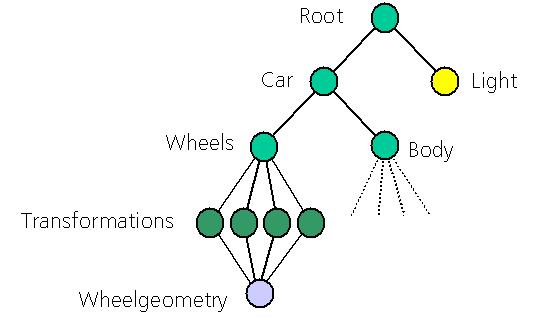
\includegraphics[width =.6\textwidth]{../figuras/scenegraph}
    \par\medskip
    Adaptado de: <http://www.opensg.org/htdocs/doc-1.8/PageScenegraph.html>. Acesso 
    em: 05/06/2017.
    \label{scenegraphexample}
\end{figure}

O grafo de cena é utilizado para gerenciar o posicionamento dos objetos da aplicação e 
também para controlar a renderização destes através da chamada do método \textit{draw}. 
Na versão orientada a objetos do motor, o grafo de cena é divido em duas classes diferentes, uma 
para armazenar a raiz do grafo e a câmera utilizada, e outra para armazenar os dados de 
um nó do grafo, esta segunda classe possui a maioria das propriedades e funcionalidades 
do grafo de cena. Além do método \textit{draw}, um nó pode criar um nó filho, 
armazenando-o em um vetor de filhos. Outras propriedades do nó incluem: um programa de 
\textit{shader}, um objeto, um ponteiro para o nó pai e uma \textit{string} de 
identificação.

Na abordagem orientada a dados, as duas classes que representam o grafo de cena foram 
reduzidas a somente uma estrutura, que contém \textit{arrays} contíguos das mesmas 
propriedades da versão orientada a objetos, conforme discutido na 
seção~\ref{proposalcap}, essa estrutura segue o \textit{layout} de armazenamento de 
dados SoA. A raiz do grafo 
sempre será o primeiro elemento em todos os \textit{arrays}, a câmera foi desacoplada 
do grafo e seu armazenamento foi movido para outra parte. O vetor de filhos foi 
removido e a hierarquia é definida somente pela referência ao nó pai de cada nó.

O método \textit{draw} é o principal do grafo de cena, por ser 
utilizado no loop principal da aplicação para controlar a 
renderização do grafo. O código~\ref{oodraw} apresenta a 
implementação do método \textit{draw} na versão OO do motor.

\begin{lstlisting}[frame=single, caption={Método draw versão OO}, label=oodraw]
01  void draw() {
02      if (object == nullptr) {
03          throw RenderException("Nó sem objeto");
04      }
05      if (shaderProgram == nullptr) {
06          shaderProgram = getProgramFromParent();
07          if (shaderProgram == nullptr) {
08              throw RenderException("Nó sem shader");
09          }
10     }
11     Matrix4 modelMatrix = this->getModelMatrix();
12     shaderProgram->use();
13     shaderProgram->setUniform("Matrix", modelMatrix);
14     object->drawObject();
15     if (!children.empty()){
16         int i;
17         for (i = 0; i < (int)children.size(); i++) {
18             children[i]->draw();
19         }
20     }
21 }
\end{lstlisting}

As linhas 2 e 5 contém instruções com condicionais verificando o 
estado do nó, a primeira para verificar se o nó está sem objeto, 
e a segunda para verificar sem o nó está sem shader. Na linha 11 
é chamado um método recursivo para se obter a matriz de 
transformação do nó a partir do nó pai, sendo que a matriz de 
transformação do nó raiz é a matriz identidade.

Nas linhas 12 e 13 são chamados dois métodos do programa de shader, 
o primeiro para especificar ao \textit{openGL} que aquele programa de shader 
será utilizado. O segundo método altera o valor da variável 
uniforme "Matrix" contida no programa para o valor da matriz 
de transformação calculado para o nó.

Na linha 14 é chamado o método \textit{drawObject} do objeto, 
que é um \textit{wrapper} para a função de renderizar triângulos 
do \textit{openGL}, a qual necessita dos dados da malha vinculada 
ao objeto. A linha 15 contém uma condicional para verificar o 
estado do vetor de filhos, e se o nó possuir pelo menos um filho, 
é iniciado o processo recursivo de renderização dos filhos.

O código~\ref{oddraw} apresenta o método \textit{draw} para a 
versão OD do motor, alterado de acordo com as mudanças feitas nas 
estruturas do motor. Para evitar que muitas propriedades das 
entidades sejam utilizadas em uma transformação, o método foi 
dividido em três partes diferentes: cálculo das coordenadas locais 
(coordenadas do objeto), cálculo das coordenadas globais (coordenadas 
do mundo), e a renderização propriamente dita. Nota-se que todas 
as subfunções consistem em loops que percorrem as propriedades de 
todas as entidades, além disso, o elemento 0 de todas as 
propriedades nunca é processado por ser reservado para a raiz.

\begin{lstlisting}[frame=single, caption={Método draw versão OD}, label=oddraw]
01  void calcularLocais(transl, rots, escalas, out_locais) {
02      for (i = 1; i < nObjetos; i++) {
03          out_locais[i] =  math::translate(transl[i]) *
04                           rots[i].toMatrix() *
05                           math::scale(escalas[i]);
06      }
07  }
08  void calcularGlobais(locais, pais, out_globais) {
09      for (i = 1; i < nObjetos; i++) {
10          out_globais[i] = out_globais[pais[i]] * locais[i];
11      }
12  }
13  void renderizarNos(globais, shaders, malhas) {
14      for (i = 1; i < nObjetos; i++) {
15          glUseProgram(shaders[i].programID);
16          glUniformMatrix4fv(shaders[i].matrixID, ..., globais[i]);
17          glBindVertexArray(malhas[i].vaoId);
18          glDrawArrays(GL_TRIANGLES, 0, meshes[i].nVertices);
19      }
20  }
21
22  void draw() {
23      calcularLocais(...);
24      calcularGlobais(...);
25      renderizarNos(...);
26  }
\end{lstlisting}

O cálculo das coordenadas locais (linhas 01 a 07) é feito 
multiplicando-se a translação, rotação e escala de cada objeto e 
armazenando os valores resultantes no vetor de saída 
\textit{out\_locais}. O cálculo das coordenadas globais (linhas 08 a 
12) é feito com as coordenadas locais calculadas na etapa anterior 
e o vetor de pais, responsável por manter a hierarquia do grafo. O 
cálculo em si é um \textit{loop} simples que multiplica a matriz de 
coordenadas locais do nó pela matriz de coordenadas globais do pai. 

O \textit{loop} sequencial para o cálculo de globais funciona pois 
o grafo e sua hierarquia é construído de tal forma que um nó nunca 
terá um número identificador maior do que os dos seus filhos. Desta 
maneira, apenas globais já processadas serão acessadas (a global 
do nó raiz é a matriz identidade).

A última subfunção \textit{renderizarNos} não contém processamento 
de dados, apenas chamadas de funções do \textit{openGL} para renderizar 
os objetos dos nós do grafo. Esta última etapa utiliza três propriedades 
dos nós: a matriz de coordenadas globais, os dados do shader e dados da 
malha.

\subsection{Otimizações de Renderização}

Como o processo de renderização é computacionalmente caro, é necessário que esse 
processo seja o mais otimizado o possível. Até mesmo simples otimizações podem causar 
um impacto considerável no desempenho da renderização. 

Dentre outras, há duas otimizações de renderização que são utilizadas neste trabalho: 
\textit{backface culling} e \textit{frustum culling}.

O \textit{backface culling} é uma técnica que elimina um dos dois lados de uma face. 
Como em aplicações 3D os objetos consistem em malhas que por sua vez são um conjunto 
de faces adjacentes, apenas um dos lados dessas faces são vistos, chamado de parte de 
fora das malhas. O interior dos objetos, chamado de parte de dentro, não é visto pelo 
espectador, por isso não há motivo em renderizá-lo, o \textit{backface culling} é 
encarregado de eliminar essa parte do interior~\cite{hughes2014computer}.

O \textit{frustum culling} é a remoção total ou parcial dos objetos que estão fora do 
\textit{frustum} de visualização da câmera. Uma cena pode ser potencialmente extensa e 
conter objetos com formas complexas, por isso é importante que os parâmetros que 
definem as dimensões do \textit{frustum} de visualização sejam adequadamente ajustados, 
para que objetos muito distantes ou fora do ângulo de visualização da câmera não sejam 
renderizados.

\section{Componente Físico}

O componente físico do motor consiste nas estruturas dos objetos, e métodos para 
controlar suas atualizações, alterar os valores das velocidades e acelerações, e 
calcular colisões dentro de uma caixa. No \textit{loop} de jogo descrito na 
seção~\ref{gameloopsec}, o componente físico tende a ser o primeiro componente 
do motor a ser atualizado na etapa de processamento do \textit{loop}, logo 
após a detecção e gerenciamento de \textit{inputs} do jogador.

Na versão OO do motor, a classe de objeto contém todos os seus dados, as propriedades 
relacionadas à geometria, que são a translação, rotação e escala, à parte visual, 
constituída pela malha, e à parte física, constituída pela velocidade e aceleração. 
Além das propriedades, a classe de objetos possui quatro métodos principais: 
chamada para a renderização da malha, cálculo da matriz de transformação, 
atualização do objeto e verificação de colisão com uma caixa. O gerenciador de objetos, 
apresentado como uma das classes com sufixo \textit{Manager} na figura~\ref{umlengine}, 
é a classe responsável por administrar a atualização dos objetos e colisões contra a 
caixa.
%\quad

O código~\ref{ooupdate} contém os dois métodos utilizados para atualizar os objetos 
da cena. O primeiro é o método \textit{update}, contido na classe de objetos, que atualiza 
as propriedades da classe relacionadas à geometria e física. O segundo método 
\textit{updateObjects} é chamado pela classe \textit{ObjectManager} que controla a 
atualização dos objetos. O método simplesmente percorre o conjunto de objetos e 
invoca o método \textit{update} de cada um deles.

\begin{lstlisting}[frame=single, caption={Métodos para atualização dos objetos versão OO}, label=ooupdate]
01 virtual void update() {
02   math::clampVector(speed + accel, MIN_SPEED, MAX_SPEED);
03
04   translation = translation + speed;
05
06   Quaternion Y = Quaternion(speed.x, (.0f, 1.0f, .0f, 1.0f));
07   Quaternion X = Quaternion(-speed.y, (1.0f, .0f, .0f, 1.0f));
08
09   rotation = X * Y * rotation;
10 }
11 void updateObjects(vector<Object*> objects) {
13   auto it = objects.begin();
14
15   for(it = objects.begin(); it != objects.end(); it++) {
16       it->update();
17   }
18 }
\end{lstlisting}

\newpage

\begin{lstlisting}[frame=single, caption={Métodos para atualização dos objetos versão OD}, label=odupdate]
01  void updateSpeeds(Vector3* speeds, Vector3* accels) {
02    for (i = 1; i < totalObjects; i++) {
03      math::clampVector(
04          speeds[i] + accels[i], 
05          MIN_SPEED, 
06          MAX_SPEED);
07    }
08  }
09  void updateTranslations(Vector3* transls, Vector3* speeds) {
10    for (i = 1; i < totalObjects; i++) {
11      transls[i] = transls[i] + speeds[i];
12    }
13  }
14  void updateRotations(Quaternion* rotations, Vector3* speeds) {
15    for (i = 1; i < totalObjects; i++) {
16      Vector3 *speed = &speeds[i]
17      Quaternion *rotation = &rotations[i]
18      Quaternion Y = Quaternion(speed.x, (.0f, 1f, .0f, 1f));
19      Quaternion X = Quaternion(-speed.y, (1f, .0f, .0f, 1f));
20
21      rotation = X * Y * rotation;
22    }
23  }
24  void update() {
25      updateSpeeds(...);
26      updateTranslations(...);
27      updateRotations(...);
28  }
\end{lstlisting}

O código~\ref{odupdate} apresenta a conversão para a versão OD. Percebe-se que a 
conversão segue o mesmo modelo aplicado para a conversão do grafo de cena na 
seção~\ref{scenegraphsection}, as propriedades do objeto foram separadas em 
\textit{arrays} contíguos e as funções foram adaptadas conforme as mudanças das 
estruturas. A função \textit{update} foi dividida em três subfunções: 
\textit{updateSpeeds}, \textit{updateTranslations} e \textit{updateRotations}, 
para atualizar as velocidades, translações e rotações respectivamente.

Os códigos~\ref{oocolision} e~\ref{odcolision} apresentam as chamadas para a função de 
verificação de colisão das versões OO e OD, respectivamente. O método \textit{colidiu} 
verifica se o vetor de translação do objeto não ultrapassou os limites da caixa, e 
inverte os valores de velocidade, caso alguma colisão tenha ocorrido, não foi utilizado 
coeficiente de absorção, ou seja, o objeto mantém a mesmo velocidade ao colidir.

\begin{lstlisting}[frame=single, caption={Chamada da verificação de colisão versão OO}, label=oocolision]
01 void calcularColisoes(Caixa caixa) {
02   auto it = objects.begin();
03
04   for(it = objects.begin(); it != objects.end(); it++) {
05       it->second->colidiu(caixa);
06   }
07 }
\end{lstlisting}

\begin{lstlisting}[frame=single, caption={Chamada da verificação de colisão versão OD}, label=odcolision]
01 void calcularColisoes(transls, speeds, caixa) {
02   for(i = 1; i < totalObjects; i++) {
03       colidiu(transls[i], speeds[i], caixa);
04   }
05 }
\end{lstlisting}

\section{Gerenciador de Recursos}

O gerenciador de recursos consiste em uma interface unificada que serve como conexão 
entre o conteúdo técnico da aplicação, nesse caso o motor de jogos e todos os seus 
módulos, e o conteúdo criativo, conhecido como \textit{assets}, o qual é constituído 
de malhas, animações, sons, música, planos de fundo, fontes, texturas, e qualquer outro 
tipo de conteúdo que seja julgado necessário. Além dos \textit{assets}, há também 
outros tipos de dados que são gerenciados por este componente, que são \textit{inputs} 
do motor de jogos, como scripts, cenas e \textit{shaders}.

A função dessa interface é garantir acesso a esses \textit{assets} e \textit{inputs} 
do motor de jogos a partir da utilização do sistema de arquivos do sistema operacional 
no qual a aplicação está sendo executada, onde esse conteúdo externo está armazenado. 
O acesso ao sistema de arquivos já é fornecido por bibliotecas da linguagem de 
programação. Cabe então ao gerador de recursos fornecer funções com um maior nível de 
abstração que utiliza essas chamadas ao sistema de arquivos disponibilizadas pela 
linguagem, esse processo é conhecido como criação de um \textit{wrapper}. 

Algumas das funcionalidades presentes na API de acesso ao sistema de arquivos 
incluem~\cite{gregory2009game}:
\begin{itemize}
    \item Manipulação de nomes de arquivos e caminhos de diretórios,
    \item Abrir, fechar, ler e escrever arquivos individuais,
    \item Listar os conteúdos de um diretório,
    \item Gerenciamento de pedidos de I/O assíncronos
\end{itemize}

Além dessas funções, é também da responsabilidade do gerenciador de recursos garantir 
que apenas uma cópia de cada arquivo carregado no sistema exista, economizando o uso 
da memória, a qual é escassa. Por exemplo, vários objetos presentes em uma cena podem 
compartilhar uma mesma malha, então mesmo que exista mais de um objeto que utilize a 
mesma malha, somente uma cópia desta é necessária estar carregada no sistema.

Para o trabalho proposto, o gerenciador de recursos possui três funcionalidades 
principais:
\begin{itemize}
    \item Carregar malhas externas,
    \item Carregar \textit{shaders},
    \item Garantir a singularidade de cada um dos recursos carregados no sistema.
\end{itemize}

Para carregar malhas externas, o gerenciador de recursos possui um \textit{parser} 
de arquivos no formato OBJ, um formato de arquivo para definição de geometria. Um 
arquivo OBJ contém as posições de cada vértice, as coordenadas de textura, as normais 
de cada vértice e a lista de faces que compõem o objeto. As faces são triangulares, e 
cada face é constituída de três triplas de índices, o primeiro índice é de um dos 
vértices do triângulo, o segundo índice é da coordenada de textura do vértice e o 
terceiro índice é a normal do vértice.

Para carregar os \textit{shaders}, além de especificar o caminho do diretório onde o 
\textit{shader} se encontra, há um outro parâmetro que especifica qual é o tipo do 
\textit{shader} que está sendo carregado, isso é necessário para que a sua compilação 
seja adequada.

O gerenciamento dos recursos na primeira versão do motor é feito pelas classes 
\textit{Managers} conforme discutido na seção~\ref{proposalcap}. Os \textit{Managers}
gerenciam o armazenamento dos recursos e fornece uma interface para manipulá-los, 
o \textit{Manager} dos objetos por exemplo fornece métodos para atualizar os 
objetos e calcular as colisões.

Na segunda versão do motor, os métodos das classes foram separados 
entre métodos para criação de recursos e métodos utilizados no ciclo 
principal. Os métodos de criação de recursos foram movidos para uma 
interface separada e incluem: carregamento 
de arquivos externos, compilação de \textit{shaders} e criação de 
objetos e nós. Os métodos do ciclo principal são os métodos que 
sofreram alterações entre as duas abordagens do motor e foram 
discutidos nas seções anteriores. Como as estruturas da segunda 
versão contém \textit{arrays} com todos os dados dos objetos 
presentes na cena, não foi necessário uma segunda estrutura 
para gerenciar o seu armazenamento.

\section{Considerações Finais do Capítulo}

Foram apresentadas duas abordagens de implementação para 
um motor de jogos, uma seguindo o modelo de desenvolvimento 
com programação orientada a objetos, e outra utilizando uma 
abordagem com modelagem orientada a dados conforme discutido 
na seção~\ref{secdataorienteddesign}.
Além do desenvolvimento de uma segunda versão, as estratégias 
utilizadas para a conversão das as estruturas e métodos entre 
as duas abordagens foram discutidas.

Como um motor de jogos é apenas um recurso utilizado para a criação de uma aplicação 
gráfica, foi necessário desenvolver uma aplicação idêntica para as 
duas versões do motor, com o objetivo de investigar a 
modelagem orientada a dados como uma forma de otimização de 
desempenho, comparando as duas abordagens.

Todas as operações matemáticas apresentadas e explicadas na seção~\ref{secmathconcepts} 
são utilizadas em uma biblioteca matemática, essa por sua vez é extensivamente 
utilizada nos outros módulos do motor. As funcionalidades de cada uma das estruturas 
utilizadas foram listadas. Além disso, algumas funcionalidades e convenções 
relacionadas com nenhuma das estruturas também foram listadas.

O componente gráfico é uma parte extensa do motor de jogos e que precisa lidar com 
vários fatores diferentes. Esses fatores foram apresentados e juntamente com eles 
quais foram as decisões tomadas para a implementação ou gerenciamento de cada um.

Foi apresentado o conceito de uma câmera, e possíveis configurações diferentes que 
esta pode ter. Também foi apresentada uma estrutura para lidar com a hierarquia de 
objetos de uma cena e suas propriedades, o grafo de cena, e duas técnicas de otimização 
de renderização utilizadas neste trabalho.

Além do componente gráfico, foi implementado um componente físico 
para lidar com atualização de objetos e colisões contra uma caixa.
Por fim, um outro componente foi apresentado, o gerenciador de 
recursos, que fornece uma interface para acessar todo o conteúdo 
criativo, que é externo ao motor de jogos.

\chapter{Análises e Resultados}
\label{resultscap}

Neste capítulo serão apresentados os resultados obtidos na 
comparação entre as duas versões do motor. A parte comparada 
entre as duas versões consiste nos métodos utilizados no 
ciclo principal da aplicação, que são as funções chamadas 
uma vez por objeto em todos os quadros, o que significa que 
quase todo o processamento feito no CPU é realizado através 
destas funções. Além da análise de desempenho, será 
discutido quais foram os principais desafios para a 
conversão entre as abordagens.

Para cada uma das funções, foi medido o tempo médio de execução 
para 1000 execuções da função, variando a quantidade de objetos 
na cena entre 100 e 3200 para analisar 
a escalabilidade de cada uma das abordagens. Para determinar o 
limitante superior da entrada do programa, retirou-se o limite de 
FPS da aplicação e o número de objetos foi incrementado até se chegar 
em 60 FPS, que é considerado a taxa de quadros por segundo mínima no 
atual mercado de jogos, a taxa de FPS da aplicação chegou a esse 
número com 3200 objetos sendo renderizados por quadro na cena.

Seguindo o modelo de testes feito por~\citeonline{Fontana2017} 
discutido no capítulo~\ref{relatedworkscap}, as duas versões 
do motor foram testadas em dois cenários, cada um com um 
problema diferente. O primeiro problema possui um mal padrão 
de acesso à memória, o que significa que os dados necessários 
a um procedimento não estão armazenados próximos um ao outro 
na memória. O segundo problema por outro lado, possui um bom 
padrão de acesso à memória. A descrição detalhada de cada 
problema será feita nas próximas seções do capítulo.

Para a execução dos testes, foram utilizadas as seguintes 
especificações técnicas: \\

\begin{itemize}
    \item Sistema operacional Linux x64 kernel 4.12.8-2-ARCH
    \item Processador Intel(R) Core(TM) i5-4440 CPU @ 3.10GHz com 4 núcleos
    \item Memória RAM Kingston 8192 MB velocidade: 1600 MT/s
    \item GPU GeForce GTX 760 2GB 
    \item OpenGL 3.3.0
    \item C++ 11
    \item GCC 7.2.0
\end{itemize}

Para evitar interferência nas medidas de desempenho, as otimizações 
do compilador foram desativadas. Além disso, como a intenção deste 
trabalho é investigar otimizações para a comunicação entre o 
processador e a memória, as funções que realizam comunicação entre 
o CPU e o GPU ou processamento no GPU também foram desativadas
para o cálculo de tempo da função \textit{draw}.

\section{Problema A: renderização de objetos sem hierarquia}

No problema A os objetos presentes na cena não possuem uma real 
hierarquia entre eles, todos os nós do grafo de cena são filhos 
do nó raiz. Em um cenários destes um grafo de cena normalmente 
não seria necessário, porém a estrutura foi mantida para 
demonstrar o impacto do acesso à memória no desempenho.

Este cenário é o melhor possível para a versão OO do motor, pois 
a execução do método \textit{draw} se torna semelhante entre as 
duas abordagens, alterando somente a maneira como os dados estão 
alocados na memória. Analisando o código~\ref{oddraw} pode-se 
observar que o método \textit{draw} para a versão OD do motor 
utiliza uma quantidade considerável de propriedades dos nós 
para renderizá-los, isso causa um impacto negativo no desempenho
da segunda versão, que usa o modelo de alocação \textit{Sructure 
of Arrays}. 

\begin{table}[h!]
\centering
\caption{Tempo médio de execução das funções em milissegundos no problema A para a versão OO.}
\label{oodv1table}
\begin{tabular}{c|cc|cc|cc}
\cline{2-7}
                                       & \multicolumn{2}{c|}{Draw}                                     & \multicolumn{2}{c|}{Att. objetos}                              & \multicolumn{2}{c}{Verif. colisões}                \\ \hline
\multicolumn{1}{l|}{Número de objetos} & \multicolumn{1}{l}{Média} & \multicolumn{1}{l|}{Desv. padrão} & \multicolumn{1}{l}{Média} & \multicolumn{1}{l|}{Desv. padrão} & Média           & \multicolumn{1}{l}{Desv. padrão} \\ \hline
100                                     & \textbf{0.51}              & 0.35                             & 0.03                    & 0.006                                 & 0.005           & 0.02                              \\ \hline
200                                     & \textbf{1.00}              & 0.001                            & 0.08                    & 0.002                                 & 0.01            & 0.005                             \\ \hline
400                                     & \textbf{1.86}              & 0.05                             & 0.18                    & 0.05                                  & 0.02            & 0.03                              \\ \hline
800                                     & \textbf{3.69}              & 0.06                             & 0.26                    & 0.04                                  & 0.032           & 0.04                              \\ \hline
1600                                    & \textbf{7.35}              & 0.4                              & 0.50                    & 0.02                                  & 0.066           & 0.1                               \\ \hline
3200                                    & \textbf{14.72}             & 0.2                              & 0.99                    & 0.01                                  & 0.132           & 0.06                              \\ \hline
\end{tabular}
\end{table}

\begin{table}[h!]
\centering
\caption{Tempo médio de execução das funções em milissegundos no problema A para a versão OD.}
\label{dodv1table}
\begin{tabular}{c|cc|cc|cc}
\cline{2-7}
                                       & \multicolumn{2}{c|}{Draw}                                     & \multicolumn{2}{c|}{Att. objetos}                              & \multicolumn{2}{c}{Verif. colisões}                \\ \hline
\multicolumn{1}{l|}{Número de objetos} & \multicolumn{1}{l}{Média} & \multicolumn{1}{l|}{Desv. padrão} & \multicolumn{1}{l}{Média} & \multicolumn{1}{l|}{Desv. padrão} & Média           & \multicolumn{1}{l}{Desv. padrão} \\ \hline
100                                     & 0.62                       & 0.05                              & \textbf{0.02}              & 0.005                             & $\bm{6 x 10^{-3}}$   & $7 x 10^{-3}$                      \\ \hline
200                                     & 1.04                       & 0.01                              & \textbf{0.04}              & 0.003                             & \textbf{0.001}           & $2 x 10^{-3}$                      \\ \hline
400                                     & 1.96                       & 0.05                              & \textbf{0.11}              & 0.01                              & \textbf{0.002}           & 0.001                              \\ \hline
800                                     & 3.84                       & 0.05                              & \textbf{0.22}              & 0.03                              & \textbf{0.004}           & 0.002                              \\ \hline
1600                                    & 7.65                       & 0.06                              & \textbf{0.45}              & 0.01                              & \textbf{0.008}           & $2 x 10^{-3}$                      \\ \hline
3200                                    & 15.28ms                    & 0.1                               & \textbf{0.91}              & 0.01                              & \textbf{0.016}           & $6 x 10^{-3}$                      \\ \hline
\end{tabular}
\end{table}

As tabelas~\ref{oodv1table} e~\ref{dodv1table} mostram os tempos 
médios de execução dos três métodos para as versões OO e OD, 
respectivamente. O método \textit{draw} é consideravelmente mais 
custoso do que os outros dois métodos, pois é a etapa na qual a 
maior parte das multiplicações de matrizes ocorrem. Analisando os 
valores do desvio padrão, pode-se concluir que não houve muita 
variação de tempo para todas as funções em todos os casos.

Conforme mencionado, a versão OD sofreu impacto no desempenho da 
função \textit{draw}, pois além de utilizar a maior quantidade de 
propriedades das entidades, a subfunção de calcular as coordenadas 
globais acessa em todas as iterações desta o elemento 0 do vetor 
de coordenadas globais, realizando uma leitura não sequencial do 
vetor. Nota-se que é a única função a qual a versão OD obteve um 
resultado inferior, tendo um desempenho em média 4\% mais lento em 
comparação à versão OO.

A função de atualização de objetos utiliza uma quantidade menor 
de propriedades em relação à função de renderização. As tabelas 
indicam que o tempo médio de execução das duas abordagens é 
quase idêntico.

A função de detecção de colisão utiliza somente duas propriedades 
das entidades. O tempo médio de execução desta função na versão 
OD do motor foi consideravelmente menor do que na versão OO, tendo 
um desempenho com uma ordem de magnitude mais rápido em todos os 
casos. Isso demonstra como o desempenho para essa abordagem é 
inversamente proporcional ao número de propriedades utilizadas.

Uma outra medida de desempenho comumente utilizada, a qual foi 
mencionada na seção~\ref{gameloopsec}, é a taxa de quadros por 
segundo, ou FPS. Por apontar quantos quadros são renderizados 
por segundo, o FPS pode ser utilizado para medir o desempenho 
geral das aplicações pois calcula quantos ciclos principais 
a aplicação é capaz de executar em um segundo.

\begin{table}[h!]
\centering
\caption{Taxa média de FPS no problema A para as duas versões}
\label{fpsv1table}
\begin{tabular}{c|cc|cc}
\cline{2-5}
                                       & \multicolumn{2}{c|}{Versão OO}                                & \multicolumn{2}{c}{Versão OD}                                \\ \hline
\multicolumn{1}{l|}{Número de objetos} & \multicolumn{1}{l}{Média} & \multicolumn{1}{l|}{Desv. padrão} & \multicolumn{1}{l}{Média} & \multicolumn{1}{l}{Desv. padrão} \\ \hline
100                                    & \textbf{2561.90}          & 130.29                            & 1615                      & 4.59                             \\ \hline
200                                    & \textbf{1403.18}          & 26.63                             & 874.45                    & 3.20                             \\ \hline
400                                    & \textbf{726.54}           & 2.38                              & 457.90                    & 2.71                             \\ \hline
800                                    & \textbf{375.81}           & 2.62                              & 232.27                    & 3.54                             \\ \hline
1600                                   & \textbf{191.00}           & 0.42                              & 118.00                    & 2.37                             \\ \hline
3200                                   & \textbf{96.54}            & 0.65                              & 60.00                     & 0.00                             \\ \hline
\end{tabular}
\end{table}

A tabela~\ref{fpsv1table} apresenta as taxas médias de FPS obtidas em execuções 
de 30 segundos para as duas versões, variando a quantidade de objetos em cena. 
Nota-se que com 3200 objetos em cena a versão OD executa a uma taxa fixa de 
60 FPS, considerado a taxa mínima para jogos modernos. Visto que o método 
\textit{draw} é o que possui o maior tempo de execução das funções principais e 
que esse é o método que a versão OO tem vantagem no problema A, era esperado 
que esta obtivesse a vantagem no teste de FPS.

\newpage

\begin{figure}[h!]
    \centering
    \captionof{figure}{Gráficos comparativos do problema A para os 
    três métodos do ciclo principal das duas abordagens.}
    \begin{subfigure}[b]{\textwidth}
        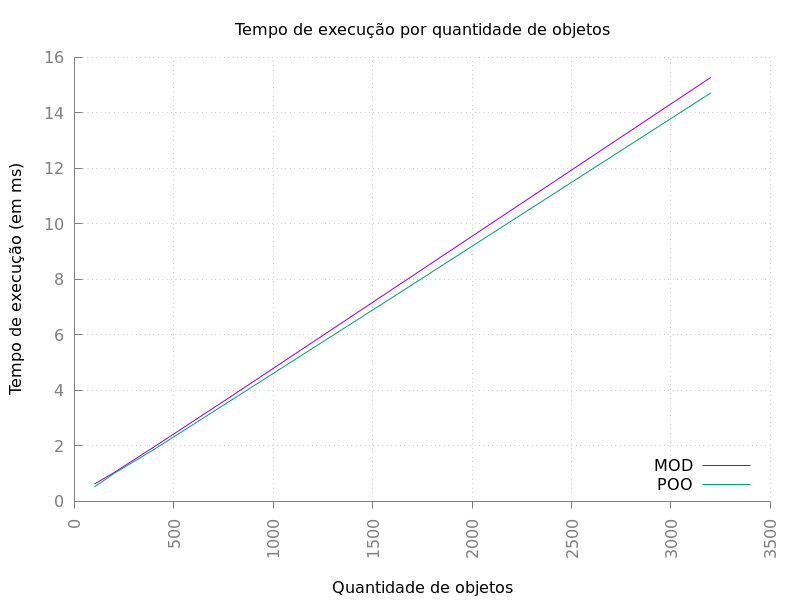
\includegraphics[width=\textwidth]{../figuras/drawv1graph}
        \caption{Método \textit{draw}.}
        \label{drawv1graph}
    \end{subfigure}
    \begin{subfigure}[b]{\textwidth}
        \begin{subfigure}[b]{.5\textwidth}
            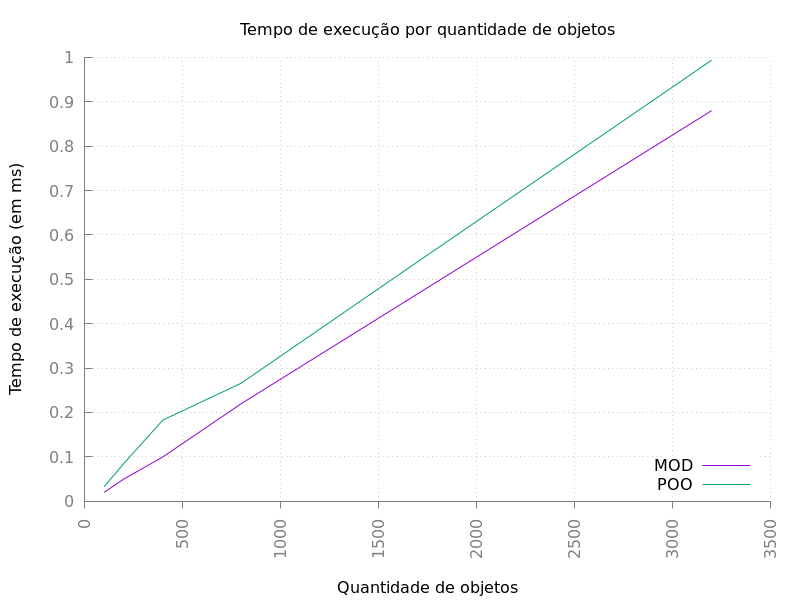
\includegraphics[width=\textwidth]{../figuras/updatev1graph}
            \caption{Método \textit{update}}
            \label{updatev1graph}
        \end{subfigure}
        \begin{subfigure}[b]{.5\textwidth}
            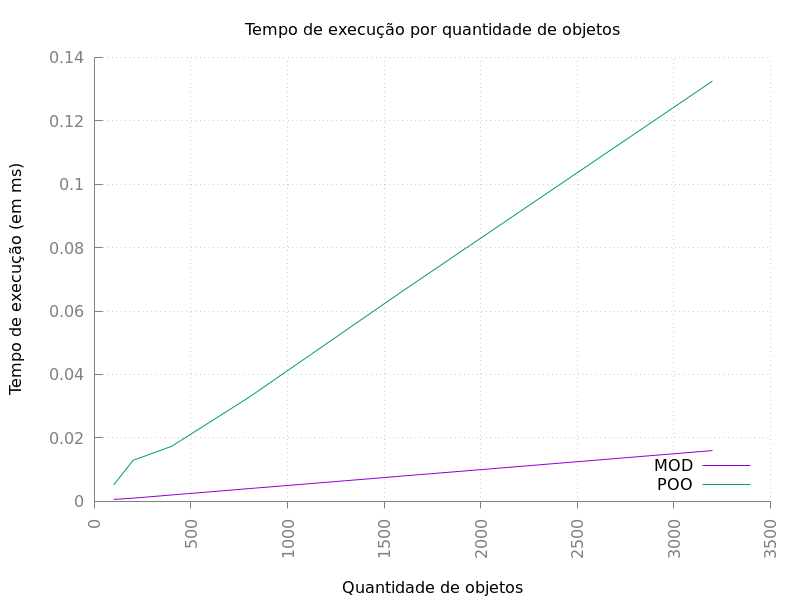
\includegraphics[width=\textwidth]{../figuras/colisionv1graph}
            \caption{Método de vef. de colisão}
            \label{colisionv1graph}
        \end{subfigure}
    \end{subfigure}
    \par\medskip
    \label{v1graphs}
\end{figure}

Os gráficos~\ref{drawv1graph},~\ref{updatev1graph} 
e~\ref{colisionv1graph} corroboram o comportamento descrito nessa 
seção, onde o ganho de desempenho da versão OD aumenta conforme 
o número de propriedades requeridas para uma função diminui.

\begin{figure}[h!]
    \centering
    \captionof{figure}{Gráfico comparativo das taxas de FPS no problema A.}
    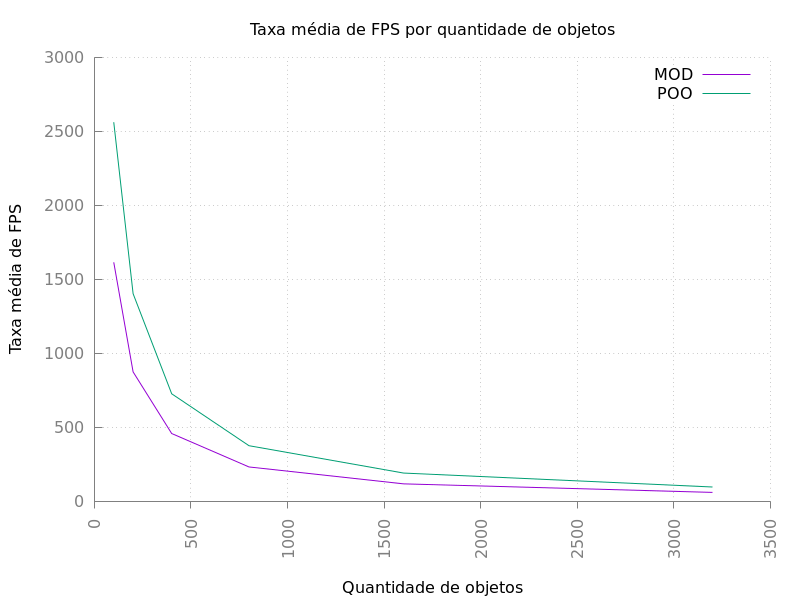
\includegraphics[width =\textwidth]{../figuras/fpsv1}
    \par\medskip
    \label{fpsv1graph}
\end{figure}

A figura~\ref{fpsv1graph} contém o gráfico correspondente à tabela~\ref{fpsv1table},
nota-se que a discrepância entre as duas versões é consideravelmente maior para 
poucos objetos em cena. Além disso a versão OO foi capaz de superar a versão 
OD em todos os casos, apesar de apresentar valores mais altos de desvio padrão. 
Para todos os casos de teste, a versão OO obteve uma taxa de fps em média 37\% 
maior do que a versão OD no problema A.

\section{Problema B: renderização de objetos com quatro níveis de hierarquia}

No problema B os objetos da cena seguem um padrão de hierarquia, 
diferentemente do problema A, onde todos os nós do grafo de cena 
são filhos do nó raiz. A hierarquia construída no problema B segue 
um padrão no qual uma árvore é formada a cada quatro objetos onde 
cada objeto está em um nível diferente da árvore. A quantidade de 
níveis de hierarquia foi julgada factível pois um objeto com 
quatro níveis de hierarquia não é algo incomum em jogos 3D modernos.

\begin{figure}[h]
    \centering
    \captionof{figure}{Esquema de hierarquia de nós do problema B.}
    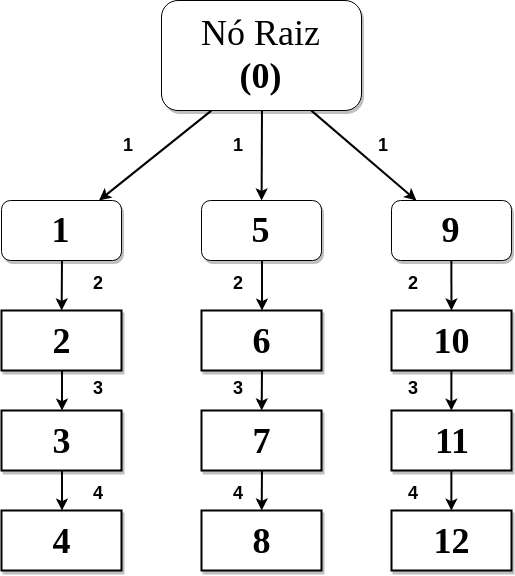
\includegraphics[width =.7\textwidth]{../figuras/problemBscheme}
    \par\medskip
    Fonte: autoria própria
    \label{problemBscheme}
\end{figure}

A figura~\ref{problemBscheme} exemplifica o esquema de hierarquia 
de nós do problema B para um exemplo de entrada com 12 objetos na 
cena. Esse esquema de hierarquia diminui consideravelmente a 
eficiência do método \textit{draw} da versão OO do motor, que 
devido a sua natureza recursiva, sofre muitas interrupções no 
fluxo de execução do programa. 

\begin{table}[h!]
\centering
\caption{Tempo médio de execução das funções em milissegundos no problema B para a versão OO.}
\label{oodv2table}
\begin{tabular}{c|cc|cc|cc}
\cline{2-7}
                                       & \multicolumn{2}{c|}{Draw}                                     & \multicolumn{2}{c|}{Att. objetos}                              & \multicolumn{2}{c}{Verif. colisões}                \\ \hline
\multicolumn{1}{l|}{Número de objetos} & \multicolumn{1}{l}{Média} & \multicolumn{1}{l|}{Desv. padrão} & \multicolumn{1}{l}{Média} & \multicolumn{1}{l|}{Desv. padrão} & Média           & \multicolumn{1}{l}{Desv. padrão} \\ \hline
100                                     & 1.02                       & 0.01                             & 0.03                      & 0.002                               & 0.004           & $7 x 10^{-3}$                     \\ \hline
200                                     & 1.94                       & 0.08                             & 0.08                      & 0.003                               & 0.01            & 0.004                             \\ \hline
400                                     & 3.76                       & 0.06                             & 0.21                      & 0.01                                & 0.02            & 0.006                             \\ \hline
800                                     & 7.46                       & 0.05                             & 0.42                      & 0.03                                & 0.036           & 0.001                             \\ \hline
1600                                    & 14.93                      & 0.09                             & 0.80                      & 0.02                                & 0.064           & 0.001                             \\ \hline
3200                                    & 29.87                      & 0.14                             & 1.50                      & 0.02                                & 0.131           & 0.007                             \\ \hline
\end{tabular}
\end{table}

\begin{table}[h!]
\centering
\caption{Tempo médio de execução das funções em milissegundos no problema B para a versão OD.}
\label{dodv2table}
\begin{tabular}{c|cc|cc|cc}
\cline{2-7}
                                       & \multicolumn{2}{c|}{Draw}                                     & \multicolumn{2}{c|}{Att. objetos}                              & \multicolumn{2}{c}{Verif. colisões}                \\ \hline
\multicolumn{1}{l|}{Número de objetos} & \multicolumn{1}{l}{Média} & \multicolumn{1}{l|}{Desv. padrão} & \multicolumn{1}{l}{Média} & \multicolumn{1}{l|}{Desv. padrão} & Média           & \multicolumn{1}{l}{Desv. padrão} \\ \hline
100                                     & \textbf{0.54}              & 0.02                              &\textbf{0.03}                      & 0.002                      &$\bm{6 x 10^{-3}}$      & $2 x 10^{-4}$                     \\ \hline
200                                     & \textbf{1.04}              & 0.01                              &\textbf{0.07}                      & 0.006                      &\textbf{0.001}          & $2 x 10^{-3}$                     \\ \hline
400                                     & \textbf{1.95}              & 0.01                              &\textbf{0.18}                      & 0.01                       &\textbf{0.004}          & 0.003                             \\ \hline
800                                     & \textbf{3.85}              & 0.04                              &\textbf{0.38}                      & 0.02                       &\textbf{0.05}           & 0.03                              \\ \hline
1600                                    & \textbf{7.62}              & 0.03                              &\textbf{0.69}                      & 0.01                       &\textbf{0.008}          & $2 x 10^{-3}$                     \\ \hline
3200                                    & \textbf{15.29}             & 0.06                              &\textbf{1.31}                      & 0.01                       &\textbf{0.01}           & $2 x 10^{-3}$                     \\ \hline
\end{tabular}
\end{table}

Os resultados contidos nas tabelas~\ref{oodv2table} 
e~\ref{dodv2table} indicam que o cálculo sequencial de coordenadas 
globais na versão OD do motor é uma alternativa mais resiliente à 
mudanças na hierarquia do grafo de cena, permanecendo com um tempo 
médio de execução estável após a mudança. O método \textit{draw}
da versão OO por outro lado, teve um acréscimo considerável no 
tempo de execução, com uma média de 51\% mais lento do que a 
versão OO no problema A e a versão OD no problema B. Como a única 
diferença entre o problema A e o problema B está na hierarquia de 
nós, não houveram mudanças significativas no tempo de execução 
das funções de atualização de objetos e detecção de colisões.

\newpage

\begin{table}[h!]
\centering
\caption{Taxa média de FPS no problema B para as duas versões}
\label{fpsv2table}
\begin{tabular}{c|cc|cc}
\cline{2-5}
                                       & \multicolumn{2}{c|}{Versão OO}                                & \multicolumn{2}{c}{Versão OD}                                \\ \hline
\multicolumn{1}{l|}{Número de objetos} & \multicolumn{1}{l}{Média} & \multicolumn{1}{l|}{Desv. padrão} & \multicolumn{1}{l}{Média} & \multicolumn{1}{l}{Desv. padrão} \\ \hline
100                                    & 928.90                    & 10.35                             & \textbf{1655.81}          & 16.91                            \\ \hline
200                                    & 484.27                    & 13.74                             & \textbf{876.45}           & 16.94                            \\ \hline
400                                    & 250.09                    & 1.31                              & \textbf{460.72}           & 1.91                             \\ \hline
800                                    & 126.45                    & 1.43                              & \textbf{234.36}           & 2.18                             \\ \hline
1600                                   & 64.00                     & 0.00                              & \textbf{119.81}           & 0.38                             \\ \hline
3200                                   & 32.54                     & 0.49                              & \textbf{60.00}            & 0.00                             \\ \hline
\end{tabular}
\end{table}

A tabela~\ref{fpsv2table} contém as taxas médias de FPS, que foram calculadas da 
mesma maneira que no problema A. Comparando os resultados com a 
tabela~\ref{fpsv1table}, percebe-se que a versão OD do motor manteve uma taxa 
estável perante as mudanças na hierarquia, mantendo essencialmente os mesmos valores 
de FPS obtidos no problema A, assim como as suas funções do ciclo principal. Já a 
versão OO sofreu uma queda considerável na taxa de FPS, em consequência do aumento 
no tempo de execução da sua função de renderização do grafo.


\begin{figure}[h!]
    \centering
    \captionof{figure}{Gráfico comparativo das funções \textit{draw} das duas versões para o problema B.}
    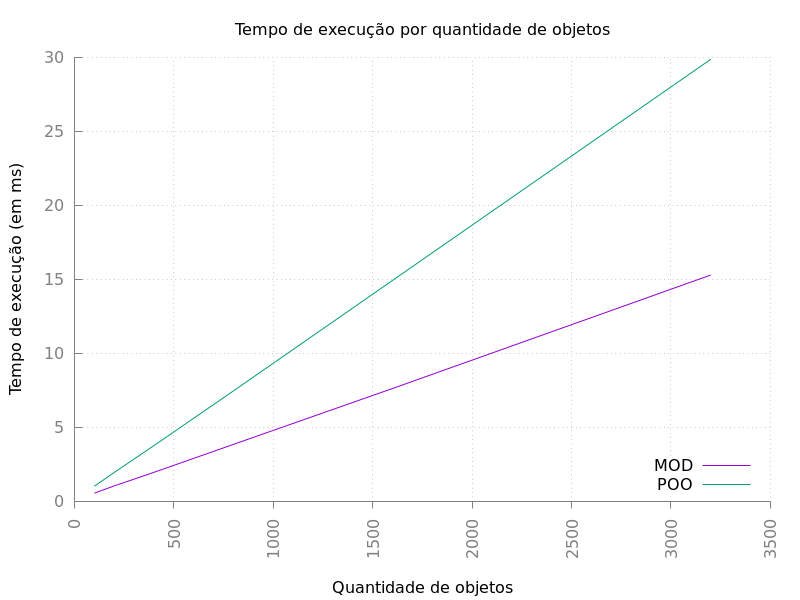
\includegraphics[width =\textwidth]{../figuras/drawv2graph}
    \par\medskip
    Fonte: autoria própria
    \label{drawv2graph}
\end{figure}

A figura~\ref{drawv2graph} contém apenas o gráfico de tempo 
para a função \textit{draw} do problema B, pois foi a única em 
que houve mudanças significativas em relação ao problema A. O 
tempo médio de execução para a versão OD permaneceu quase 
inalterado, enquanto que para a versão OO, apesar de ter 
mantido o comportamento linear, houve um acréscimo considerável.

\begin{figure}[h!]
    \centering
    \captionof{figure}{Gráfico comparativo das taxas de FPS no problema B.}
    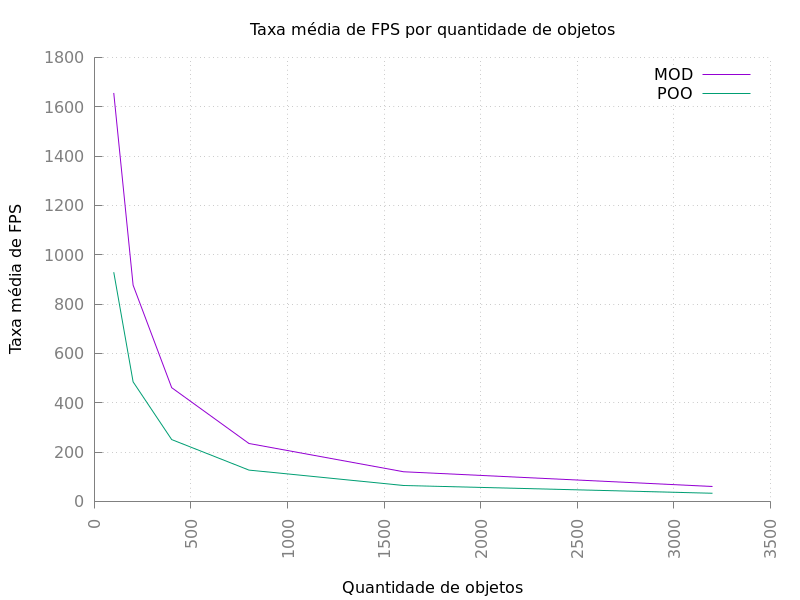
\includegraphics[width =\textwidth]{../figuras/fpsv2}
    \par\medskip
    \label{fpsv2graph}
\end{figure}

A figura~\ref{fpsv2graph} apresenta a comparação entre as taxas de FPS no problema 
B, que como pode se observar, obteve um comportamento parecido com o 
gráfico~\ref{fpsv1graph} do problema A. A diferença é que a versão OD desta vez 
foi a que obteve a maior taxa em todas as médias. A versão OO do motor também foi 
a única que obteve uma taxa inferior a 60 FPS em todos os casos de teste.
Para todos os casos de teste, a versão OD obteve uma taxa de fps em média 44\% 
maior do que a versão OO no problema B.

\section{Considerações finais do capítulo}

Neste capítulo foi testado o desempenho da modelagem orientada 
a dados, a abordagem de programação estudada neste trabalho. 
Analisando os resultados obtidos no capítulo~\ref{resultscap} e 
os conceitos discutidos na seção~\ref{secdataorienteddesign}, 
pode ser concluído que o DOD não garante uma melhora no desempenho, 
porém fornece um maior controle sobre este. Tendo o conhecimento de 
como os dados estão armazenados na memória e como estes serão 
utilizados permite ao desenvolvedor implementar os procedimentos 
da aplicação maximizando a eficiência da comunicação entre o 
CPU e a memória.

A conversão do motor da abordagem orientada a objetos para a versão 
orientada a dados apresentou alguns desafios. O primeiro, já mencionado 
no capítulo~\ref{relatedworkscap}, foi a falta de material a respeito 
de DOD. O segundo desafio foi desenvolver a versão OD com uma mentalidade 
diferente do modelo de classe e objeto, o qual os desenvolvedores de 
jogos já estão mais familiarizados.

Por fim, o maior desafio está no fato de que a abordagem orientada a dados 
requer uma constante preocupação sobre como os dados estão alocados na 
memória e como estes são acessados, o que requer uma escolha para as 
estruturas de dados utilizadas. Isso pode ser facilitado ao se 
determinar o fluxo de dados e quais são as transformações necessárias 
nestes, dividindo-as em subfunções nas quais só sejam usadas propriedades 
próximas uma da outra na memória. Porém esse processo de escolha 
das estruturas e das transformações não é trivial e em muitos casos a 
divisão não é possível, pois muitas propriedades precisam ser utilizadas ao 
mesmo tempo.

Conforme visto na seção~\ref{secdataorienteddesign}, há duas maneiras de se 
alocar os dados: o padrão AoS e o SoA, os quais possuem suas respectivas 
vantagens e desvantagens, cabendo ao desenvolvedor determinar qual padrão 
é mais adequado para cada conjunto de dados específico. Pelos 
resultados apresentados nesse capítulo, pode-se observar que o 
padrão SoA sofre uma maior penalidade no desempenho para funções 
que utilizem muitas propriedades de uma entidade.

A versão OD do motor com o padrão de armazenamento de dados 
SoA no problema A obteve um desempenho em média 4\% mais lento do
que a versão OO no método \textit{draw}, que é o que utiliza a 
maior quantidade de propriedades das entidades, um aumento 
insignificante de desempenho no método de atualização de objetos, 
o segundo a utilizar mais propriedades, e um desempenho em média 
dez vezes mais rápido no método de verificação de colisões, que 
utiliza somente duas propriedades das entidades.

Esses resultados coincidem com os obtidos e analisados 
por~\citeonline{Fontana2017}, cujo trabalho também demonstrou que 
o aumento no desempenho para a abordagem orientada a dados com o 
padrão SoA é significantemente maior para funções que utilizam 
poucas propriedades das entidades, e pode ser pior para funções que 
utilizam muitas propriedades. Não há um padrão para determinar 
um número máximo de propriedades utilizadas antes que o padrão 
SoA se torne menos eficiente. 

Conclui-se que um padrão híbrido, que utiliza 
\textit{arrays} de propriedades porém agrupa dados que são 
utilizados juntos em uma estrutura só, é o mais adequado, pois 
para alguns casos o agrupamento de propriedades em uma estrutura 
só é mais vantajoso, enquanto que para outros a separação se torna 
mais rápida, é necessário analisar cada conjunto de dados específico 
separadamente para determinar qual padrão deve ser usado. É 
importante salientar que a leitura sequencial dos \textit{arrays} 
permite um fluxo de execução ininterrupto, contribuindo 
positivamente para o desempenho conforme discutido na 
seção~\ref{secdataorienteddesign}. 

Por isso o cálculo sequencial de coordenadas globais no método 
\textit{draw} é uma alternativa mais robusta do que o algoritmo 
recursivo da versão OO do motor. O desempenho do método 
\textit{draw} nas versão OO foi em média 51\% mais lento do que a 
versão OD no problema B, no qual a única diferença em relação ao 
problema A está na hierarquia dos nós do grafo de cena.
